% sage_latex_guidelines.tex V1.20, 14 January 2017

\documentclass[Afour,sageh,times,doublespace]{sagej}

\usepackage{moreverb,url}

\usepackage{graphicx}
\usepackage{amssymb}
\usepackage{amsmath}
\usepackage[acronym]{glossaries}
\usepackage{float}
\usepackage{pgfplots}
\pgfplotsset{compat=1.16}
\usepackage{breqn}
\usepackage[colorlinks,bookmarksopen,bookmarksnumbered,citecolor=red,urlcolor=red, hidelinks]{hyperref}
\usepackage{interval}
\usepackage{tikz}
\usetikzlibrary{patterns,shapes.arrows,calc,angles,quotes,babel,arrows,arrows.meta,shapes.geometric,svg.path}
\usepackage[capitalise]{cleveref}
\usepackage{xurl}
\usepackage{uri}
\usepackage{subfig}
\usepackage{scalerel}

\definecolor{orcidlogocol}{HTML}{A6CE39}
\tikzset{
  orcidlogo/.pic={
    \fill[orcidlogocol] svg{M256,128c0,70.7-57.3,128-128,128C57.3,256,0,198.7,0,128C0,57.3,57.3,0,128,0C198.7,0,256,57.3,256,128z};
    \fill[white] svg{M86.3,186.2H70.9V79.1h15.4v48.4V186.2z}
                 svg{M108.9,79.1h41.6c39.6,0,57,28.3,57,53.6c0,27.5-21.5,53.6-56.8,53.6h-41.8V79.1z M124.3,172.4h24.5c34.9,0,42.9-26.5,42.9-39.7c0-21.5-13.7-39.7-43.7-39.7h-23.7V172.4z}
                 svg{M88.7,56.8c0,5.5-4.5,10.1-10.1,10.1c-5.6,0-10.1-4.6-10.1-10.1c0-5.6,4.5-10.1,10.1-10.1C84.2,46.7,88.7,51.3,88.7,56.8z};
  }
}

\newcommand\orcidicon[1]{\href{https://orcid.org/#1}{\mbox{\scalerel*{

\begin{tikzpicture}[yscale=-1,transform shape]
\pic{orcidlogo};
\end{tikzpicture}
}{|}}}}

\definecolor{matplotlibBlue}{HTML}{1f77b4} % blue from matplotlib color cycle
\definecolor{matplotlibOrange}{HTML}{ff7f0e} % orange from matplotlib color cycle
\definecolor{matplotlibGreen}{HTML}{2ca02c} % green from matplotlib color cycle
\definecolor{matplotlibRed}{HTML}{d62728} % red from matplotlib color cycle
\definecolor{matplotlibPurple}{HTML}{9467bd} % purple from matplotlib color cycle
\definecolor{matplotlibBrown}{HTML}{8c564b} % brown from matplotlib color cycle
\definecolor{matplotlibPink}{HTML}{e377c2} % pink from matplotlib color cycle
\definecolor{matplotlibGrey}{HTML}{7f7f7f} % grey from matplotlib color cycle
\definecolor{matplotlibYellow}{HTML}{bcbd22} % yellow from matplotlib color cycle

\tikzstyle{kernel} = [rectangle, 
minimum width=3cm, 
minimum height=1cm, 
text centered, 
text width=3cm, 
draw=black]

\tikzstyle{syncSweep} = [rectangle, 
minimum width=3cm, 
minimum height=1cm, 
text centered, 
text width=3cm, 
draw=black, 
fill=matplotlibBlue!50]

\tikzstyle{syncKernel} = [rectangle, 
minimum width=3cm, 
minimum height=1cm, 
text centered, 
text width=3cm, 
draw=black, 
fill=matplotlibOrange!50]

\tikzstyle{hybridKernel} = [rectangle, 
minimum width=3cm, 
minimum height=1cm, 
text centered, 
text width=3cm, 
draw=black, 
fill=matplotlibGreen!50]

\tikzstyle{decision} = [diamond, 
minimum width=3cm, 
minimum height=1cm, 
text centered, 
draw=black]
\tikzstyle{arrow} = [thick,->,>=stealth]

\newcommand{\walberla}{\textsc{waLBerla}}
\newcommand{\change}[1]{{\color{black} {#1}}}

\newcommand\BibTeX{{\rmfamily B\kern-.05em \textsc{i\kern-.025em b}\kern-.08em
T\kern-.1667em\lower.7ex\hbox{E}\kern-.125emX}}

\def\volumeyear{2024}

\setcounter{secnumdepth}{3}

\begin{document}

\def\journalname{The International Journal of High Performance Computing Applications}

\runninghead{Kemmler et al.}

\title{Efficiency and scalability of fully-resolved fluid-particle simulations on heterogeneous CPU-GPU architectures}

\author{Samuel Kemmler\affilnum{1,2}\orcidicon{0000-0002-9631-7349}, Christoph Rettinger\affilnum{1}\orcidicon{0000-0002-0605-3731}, Ulrich Rüde\affilnum{1,3}\orcidicon{0000-0001-8796-8599},\newline Pablo Cuéllar\affilnum{2}\orcidicon{0000-0003-2446-8065} and Harald Köstler\affilnum{1}\orcidicon{0000-0002-6992-2690}}

\affiliation{\affilnum{1}Chair for System Simulation, Friedrich-Alexander-Universität Erlangen-Nürnberg, Erlangen, Germany\\\affilnum{2}Division 7.2 for Buildings and Structures, Federal Institute for Materials Research and Testing (BAM), Berlin, Germany\\\affilnum{3}CERFACS, Toulouse, France}

\corrauth{Samuel Kemmler, Chair for System Simulation, Friedrich-Alexander-Universität Erlangen-Nürnberg, Cauerstraße 11, 91058 Erlangen, Germany}

\email{samuel.kemmler@fau.de}

\newacronym{lbm}{LBM}{Lattice Boltzmann Method}
\newacronym{dem}{DEM}{Discrete Element Method}
\newacronym{cpu}{CPU}{Central Processing Unit}
\newacronym{gpu}{GPU}{Graphics Processing Unit}
\newacronym{psm}{PSM}{Partially Saturated Cells Method}
\newacronym{mem}{MEM}{Momentum Exchange Method}
\newacronym{pdfs}{PDFs}{Particle Distribution Functions}
\newacronym{cfd}{CFD}{Computational Fluid Dynamics}
\newacronym{simd}{SIMD}{Single Instruction, Multiple Data}
\newacronym{bc}{BC}{Boundary Condition}
\newacronym{srt}{SRT}{Single Relaxation Time}
\newacronym{pd}{PD}{Particle Dynamics}
\newacronym{sm}{SM}{Streaming Multiprocessor}

\begin{abstract}
Current supercomputers often have a heterogeneous architecture using both CPUs and GPUs. At the same time, numerical simulation tasks frequently involve multiphysics scenarios whose components run on different hardware due to multiple reasons, e.g., architectural requirements, pragmatism, etc. This leads naturally to a software design where different simulation modules are mapped to different subsystems of the heterogeneous architecture. We present a detailed performance analysis for such a hybrid four-way coupled simulation of a fully resolved particle-laden flow. The Eulerian representation of the flow utilizes GPUs, while the Lagrangian model for the particles runs on CPUs. First, a roofline model is employed to predict the node level performance and to show that the lattice-Boltzmann-based fluid simulation reaches very good performance on a single GPU. Furthermore, the GPU-GPU communication for a large-scale flow simulation results in only moderate slowdowns due to the efficiency of the CUDA-aware MPI communication, combined with communication hiding techniques. On 1024 A100 GPUs, a parallel efficiency of up to 71\% is achieved. While the flow simulation has good performance characteristics, the integration of the stiff Lagrangian particle system requires frequent CPU-CPU communications that can become a bottleneck. Additionally, special attention is paid to the CPU-GPU communication overhead since this is essential for coupling the particles to the flow simulation. However, thanks to our problem-aware co-partitioning, the CPU-GPU communication overhead is found to be negligible. As a lesson learned from this development, four criteria are postulated that a hybrid implementation must meet for the efficient use of heterogeneous supercomputers. Additionally, an a priori estimate of the speedup for hybrid implementations is suggested.
\end{abstract}

\keywords{Hybrid implementation, High-performance computing, Particulate flow, Lattice Boltzmann method, Discrete element method}
\glsresetall

\maketitle

\section{introduction}

% 1. importance of TKGs and reasoning on TKGs. 
% 2. low resource languages, main main idea.
% 3. relations and limitations of current works.
% 4. summarize our solutions and contributions.

Temporal Knowledge Graphs (TKGs)~\cite{YAGO,ICEWS18,WIKI,acekg} characterize temporally evolving events, where each event, represented as ({\em subject}, {\em relation}, {\em object}), is associated with temporal information ({\em time}), e.g., ({\em Macron}, {\em reelected}, {\em French president}, {\em 2022}). TKGs has facilitated various knowledge-intensive Web applications with timeliness, such as question answering~\cite{KBQA}, product recommendation~\cite{RippleNet,TKG4Rec,TKG4Rec2,RETE}, and social event forecasting~\cite{KG4Social,DyDiff-VAE,andgan,belief,misinfo,polarization}. 

As new events are continually emerging, modern TKGs are still far from being complete. Conventionally, the TKG construction process relies primarily on information extraction from unstructured corpus~\cite{WIKI,YAGO, EventKG}, which necessitates extensive manual annotations to keep up with changing events. For instance, the recent transition from Trump to Biden as the President of the United States has not been reflected in many TKGs, highlighting the need for timely updates. This spurs research on temporal knowledge graph reasoning to automate evolving events prediction over time~\cite{TA-DistMult,Know-Evolve,Renet,RE-GCN}. Unfortunately, the problem of TKG incompleteness is particularly pronounced in low-resource languages, where it is unable to collect enough corpus and annotations to support robust TKG construction. This results in suboptimal reasoning performance and distinctly unsatisfying accuracy in predicting recent and future events.

% whose performance can degrade significantly in low-resource language TKGs that suffer from severe incompleteness over time. 
% \jingfeng{why don't people  study cross-lingual TKG previously, (i.e. use language alignment to improve TKG). Is it really helpful intuitively to use high resource language to help TKGC? For instance, is it enough to use static langauge-alignment to help KGC, ignoring the temporal information? Are those langauge-alignment changing across time?}



\begin{figure}
    \centering
    \includegraphics[width = 1.0\linewidth]{fig/task.pdf}
    \caption{An illustrative example of cross-lingual reasoning on TKGs. 1) We aim to transfer knowledge from English TKG to Japanese TKG, where the English version provides more complete information; 2) Cross-lingual alignments only cover a small ratio of entities, e.g., Apple Inc; 3) Cross-lingual alignments can be noisy and misleading, e.g., A city called Ventura is linked to new macOS Ventura at $t_2$, introducing noise for reasoning in Japanese.}
    \label{fig:illustration}
    %\vspace{-6mm}
\end{figure}

Inspired by the incompleteness issue facing low-resource languages in constructing TKGs, we introduce a novel task named Cross-Lingual Temporal Knowledge Graph Reasoning (as shown in Figure~\ref{fig:illustration}). This task aims to alleviate the reliance on supervision for TKGs in low-resource languages (referred to as the target language) by transferring temporal knowledge from high-resource languages (referred to as the source language)~\footnote{In this paper, for the sake of brevity, we interchangeably use the terms high-resource/low-resource and source/target.}. In contrast, all the existing efforts are either limited to reasoning in monolingual TKGs (usually high-resource languages, e.g., English)~\cite{TA-DistMult,Know-Evolve,Renet,RE-GCN}, or multilingual static KGs~\cite{KEnS,AlignKGC,SS-AGA}. To the best of our knowledge, cross-lingual TKG reasoning that transfers temporal knowledge between TKGs has not been investigated. 

%Motivated by this, we study a new task named {\em cross-lingual temporal knowledge graph reasoning} as shown in Figure~\ref{fig:illustration}, to alleviate the heavy dependence on supervision for any resource-poor language TKGs by distilling the temporal knowledge from resource-rich ones. Differently, all the existing efforts are either limited to reasoning in monolingual (usually high-resource languages, e.g., English) temporal KGs~\cite{TA-DistMult,Know-Evolve,Renet,RE-GCN}, or multilingual static KG~\cite{KEnS,AlignKGC,SS-AGA}, but neglecting the reasoning in a both temporal and cross-lingual manner that highly requires capturing time-evolving patterns and language discrepancy. To the best of our knowledge, this problem, regarding how to transfer cross-lingual knowledge between TKGs, has still not been formally investigated. 

% Unlike conventional TKG reasoning, 
The fulfillment of this task poses tremendous challenges in two aspects: 1) \textbf{Scarcity of cross-lingual alignment}: as the informative bridge of two separate TKGs, cross-lingual alignment is imperative for cross-lingual knowledge transfer~\cite{AlignKGC,KEnS,SS-AGA}. However, obtaining alignments between languages is a time-consuming and resource-intensive process that heavily relies on human annotations. The transfer of knowledge through a limited number of alignments is often insufficient to fully enhance the TKG in the target language. 2) \textbf{Temporal knowledge discrepancy}: the information associated with two aligned entities is not necessarily identical, especially with regards to temporal patterns. Utilizing a rough approach to equate the aligned entities at all times can result in the transfer of misleading knowledge and negatively impact performance. This becomes more pronounced when the alignments are noisy and unreliable. For example, at the time step $t_2$, a new event about operating system ``{\it Ventura}'' from Apple company occurs in the source English TKG, and meanwhile there is a noisy aligned entity ``{\it Ventura city}'' in the target Japanese TKG. Directly pulling those two entities at this point, can inevitably introduce  noise and fail to predict a set of related events in the target TKG. Therefore, it is crucial to dynamically regulate the alignment strength of each local graph structure over time in order to maximize the effectiveness of cross-lingual knowledge distillation.

% Pulling those entities together cannot augment information in target languages. Small alignment strength is beneficial in the unreliable alignment cases, otherwise the misleading knowledge transferring can even hurt the performance.

% Moreover, in a case that the alignments are not fully reliable, directly pulling the two aligned entities together 


% optimally dynamic alignment strength
% {\em Optimal alignment strength to maximize the benefits of knowledge distillation is difficult to obtain, especially in the temporal manner.} 
% In practical, although the aligned entities can share similar information, they may still differ in other perspectives, including but not limited to frequency, interactions, and temporal patterns. How to adjust the alignment strength (i.e., the distance constrains of the aligned entities in the uni-space) accordingly for different entities at different time is unclear. \zheng{Ruijie TODO: add Ventura case}Moreover, in a case that the alignments are not fully reliable, directly pulling the two aligned entities together can even hurt the performance.



% scarcity of hinders the efficient
% knowledge transfer across languages. 
% {\em Transferring knowledge through a small set of alignments is hard to augment information for all entities.} 

% Aligning the same entities across languages rely heavily on manual labeling or rule-based inference~\cite{EA1,EA2,EA3,selfKG}, which is too time-consuming and impractical to obtain the alignments covering most of the entities in target language. 

% In this paper, we study how to boost the TKG reasoning performance in low-resource languages by explicitly increasing the completeness of those TKGs in history. Instead of improving the underlying information extraction techniques in low-data regime, we propose a new task called {\em Cross-lingual Temporal Knowledge Graph Reasoning}, motivated by the facts that there exists common or complementary knowledge shared by the TKGs in different languages under similar topics. The new task aims to facilitate TKG reasoning in low-resource languages (target languages) by distilling knowledge from a corresponding TKG in high-resource language (source language)  through a small set of entity alignments as bridges~\footnote{In this paper, we interchangeably use the terminology high-resource/low-resource and source/target for briety.}. Figure~\ref{fig:illustration} provides an illustrative example of the proposed task.


% Unfortunately, recent breakthroughs in temporal knowledge graph reasoning model~\cite{TA-DistMult,Know-Evolve,Renet,RE-GCN} highly rely on the completeness of the TKGs, especially for the most recent events. 

% However, the completeness of TKGs varies a lot across different languages, even under similar topics. Conventionally, the TKG construction process relies primarily on information extraction techniques built on the unstructured corpus~\cite{WIKI,YAGO, EventKG}. Therefore, the amount of corpus and human annotations in different languages significantly influence the quality of the corresponding TKGs . 
% Therefore, automatically completing/updating TKGs has been attracting enormous interests in recently years, which aims to predict recent/future events on TKGs based on historical events~\cite{TA-DistMult,Know-Evolve,Renet,RE-GCN}, namely temporal knowledge graph reasoning~\footnote{Broadly speaking, TKG reasoning includes interpolation to predict historical events and extrapolation to predict future events. In this paper, we refer to extrapolation task as TKG reasoning, since it is more vital for time-sensitive downstream tasks.}.


% For languages with large-scale and carefully labeled corpus (we refer to as high-resource languages, e.g., English), the constructed TKGs are more comprehensive than TKGs in other languages that lack the high-quality corpus (we refer to as low-resource languages, e.g., Spanish, Slovene, Danish, etc). Such completeness discrepancy leads to distinctly uneven TKG reasoning performances in different languages, which in turn affects the quality of service of the downstream applications. 


% Compared with the traditional TKG reasoning task, the new task imposes non-trivial challenges. An intuitive solution is to construct a unified graph including two TKGs in both source and target languages, and the knowledge distillation can be fulfilled by pulling the aligned entities from two languages close to each other in the uni-space~\cite{AlignKGC,KEnS}. However, there are still two challenges to be addressed. 

% \zheng{Ruijie TODO, Place this part to related works.}
% Existing works in related areas fail to address the aforementioned challenges. Monolingual reasoning methods on static/temporal knowledge graphs~\cite{TransE,TranR,ComplEX,RotatE,TA-DistMult,Know-Evolve,Renet,RE-GCN} is incapable of the desired knowledge transferring due to the insufficient alignment modeling. Although they can be extended on the cross-lingual scenario by viewing the alignments as a new relation on the merged TKGs, the limited amount of alignments prevent them from augmenting information for most of the entities. Entity alignment methods on KGs~\cite{EA1,EA2,EA3,EA4,EA5,selfKG} can automatically enlarge the alignments by  predicting the correspondence between the two TGs. But most of them, if not all, require the relatively even completeness of two TGs to capture the structural similarities, which can not be satisfied in our case, as target TKGs are far from complete. Some recent works start to study the multilingual TK reasoning on static graphs~\cite{AlignKGC,KEnS,SS-AGA}, which similarly aim to extract knowledge from several source KGs to boost the reasoning performance in the target KG, while they still require a sufficient amount of cross-lingual alignments and totally ignore the temporal perspective in our task.

% to facilitate temporal knowledge graph reasoning in low-resource languages. 
% increase the TKG connection and target TKG capacity
% In light of the mutual benefits, we iteratively generate pseudo alignment pairs and pseudo temporal events to address the co-existing scarcity issue in both cross-lingual alignment and target TKGs. 


In this paper, we propose a novel Mutually-paced Knowledge Distillation (\model) framework, where a teacher network learns more enriched temporal knowledge and reasoning skills from the source TKG to facilitate the learning of a student network in the low-data target one. The knowledge transfer is enabled via an alignment module, which estimates entity correspondence across languages based on temporal patterns. Firstly, to alleviate the limited language alignments (\textbf{Challenge \#1}), such a knowledge distillation process is mutually paced over time. This means, on one hand, we encourage the mutually interactive learning between the teacher and student. Concretely, the alignment module between the teacher and the student learns to generate pseudo alignment between TKGs to maximally expand the upper bound of knowledge transfer. And subsequently, it empowers the student to encode more informative knowledge in target TKG, which can in turn boost the alignment module to explore more reasonable alignments as the bridge across TKGs. One the other hand, inspired by self-paced learning~\cite{spl-1,spl-2}, we make the generations as a progressively easy-to-hard process over time. We start from generating reliable pseudo data with high confidence. As time goes by, we then gradually increase the generation amount by relieving the restriction over time. Secondly, to inhibit the temporal knowledge mismatch (\textbf{Challenge \#2}), the attention module can estimate the graph alignment strength distribution over time. This is achieved by a temporal cross-lingual attention in terms of the local graph structure and temporal-evolving patterns of aligned entities. As such, it can dynamically control the negative effect and suppress noise  propagation from the source TKG. Moreover, we provide a theoretical convergence guarantee for the training objective on both initial ground-truth data and pseudo data. To evaluate \model, we conduct extensive experiments of 12 cross-lingual TKG transfer tasks in multilingual EventKG dataset~\cite{EventKG}. Our empirical results show that the \model method outperforms state-of-the-art baselines in both with and without alignment noise settings, where only $20\%$ of temporal events in the target KG and $10\%$ of cross-lingual alignments are preserved.

% To validate the effectiveness of \model, we conduct extensive experiments of 12 cross-lingual TKG transfer tasks in multilingual EventKG benchmark dataset~\cite{EventKG} . Our experimental results empirically demonstrate the superiority of the \model method over state-of-the-art baselines, ranging from static KG embedding~\cite{TransE,TransR,DistMult,RotatE}, temporal KG reasoning~\cite{TA-DistMult,Renet,RE-GCN} to multilingual KG completion~\cite{KEnS,AlignKGC,SS-AGA}, in both with and without alignment noise settings. We further conduct comprehensive ablation and hyperparameter studies to validate the effectiveness of each design choices. Moreover, we provide theoretical analysis of convergence guarantee for the training objective on both initial groundtruth data and pseudo generative data.



To sum up, our contributions are three-fold:

\begin{itemize}[leftmargin = 15pt]
    \item \textbf{Problem formulation}: We propose the cross-lingual temporal knowledge graph reasoning task, to boost the temporal reasoning performance in target TKG by transferring knowledge from source TKG;
    \item \textbf{Novel framework}: We propose a novel \model framework, which enables the mutually-paced learning between the teacher and student networks, to promote both pseudo alignments and knowledge transfer reliability. Besides, \model involves a dynamic alignment estimation across TKGs that inhibits the influence of temporal knowledge discrepancy.
    \item \textbf{Extensive evaluations}: Empirically, extensive experiments on 12 cross-lingual TKG transfer tasks in multilingual EventKG benchmark dataset demonstrate the effectiveness of \model.
\end{itemize}
% pseudo data generation technique to progressively enhance the training data. The generated pseudo alignments can help the training of the representation modules by the knowledge distillation, and in turn adding pseudo events in the target TKG can improves alignment module by providing high-quality representations. 




% interactively
% TKGs in a source language and a target language are represented by a teacher representation module and a student one into a uni-space, respectively. 
% The knowledge distillation is enabled by a cross-lingual alignment module which pulls the aligned entities close to each other and push other entities far away. 
% To address the challenge caused by the scarcity of cross-lingual alignment, 


\section{Numerical methods}\label{numerical_methods}
Generally, fully resolved coupled fluid-particle simulations consist of three modules: fluid dynamics, particle physics, and fluid-particle coupling. In this section, we introduce the background of the methods based on the work of~\citet{rettingerComparativeStudyFluidparticle2017, rettingerEfficientFourwayCoupled2022}.
\cref{fig:psm_sketch} illustrates coupled fluid-particle simulations using the \gls{psm}, as it will be explained in the upcoming sections.
\begin{figure}
  \centering
  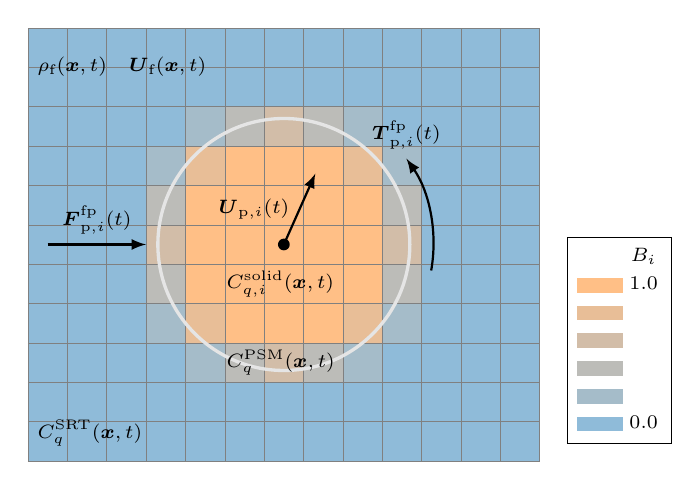
\begin{tikzpicture}[scale=1.0]
    \tikzstyle{every node}=[font=\scriptsize]
    
    % Add colors
    \definecolor{intermediate1}{HTML}{4C7993}
    \definecolor{intermediate2}{HTML}{797A72}
    \definecolor{intermediate3}{HTML}{A57C50}
    \definecolor{intermediate4}{HTML}{D27D2F}

    \colorlet{blue}{matplotlibBlue!50}
    \colorlet{i1}{intermediate1!50}
    \colorlet{i2}{intermediate2!50}
    \colorlet{i3}{intermediate3!50}
    \colorlet{i4}{intermediate4!50}
    \colorlet{orange}{matplotlibOrange!50}
    
    % Color fraction field
    \fill[blue] (0,0) rectangle (6.5,5.5);
    
    \fill[orange] (2.5,1.5) rectangle ++(1.5,2.5);
    \fill[orange] (2,2) rectangle ++(2.5,1.5);

    \fill[i1] (1.5,1.5) rectangle ++(0.5,0.5);
    \fill[i1] (1.5,3.5) rectangle ++(0.5,0.5);
    \fill[i1] (4.5,1.5) rectangle ++(0.5,0.5);
    \fill[i1] (4.5,3.5) rectangle ++(0.5,0.5);

    \fill[i1] (2,1) rectangle ++(0.5,0.5);
    \fill[i1] (4,1) rectangle ++(0.5,0.5);
    \fill[i1] (2,4) rectangle ++(0.5,0.5);
    \fill[i1] (4,4) rectangle ++(0.5,0.5);

    \fill[i2] (1.5,2) rectangle ++(0.5,0.5);
    \fill[i2] (1.5,3) rectangle ++(0.5,0.5);
    \fill[i2] (4.5,2) rectangle ++(0.5,0.5);
    \fill[i2] (4.5,3) rectangle ++(0.5,0.5);

    \fill[i2] (2.5,1) rectangle ++(0.5,0.5);
    \fill[i2] (3.5,1) rectangle ++(0.5,0.5);
    \fill[i2] (2.5,4) rectangle ++(0.5,0.5);
    \fill[i2] (3.5,4) rectangle ++(0.5,0.5);

    \fill[i3] (1.5,2.5) rectangle ++(0.5,0.5);
    \fill[i3] (4.5,2.5) rectangle ++(0.5,0.5);
    \fill[i3] (3,1) rectangle ++(0.5,0.5);
    \fill[i3] (3,4) rectangle ++(0.5,0.5);

    \fill[i4] (2,1.5) rectangle ++(0.5,0.5);
    \fill[i4] (4,1.5) rectangle ++(0.5,0.5);
    \fill[i4] (2,3.5) rectangle ++(0.5,0.5);
    \fill[i4] (4,3.5) rectangle ++(0.5,0.5);
    
    \draw[step=0.5,gray,very thin] (0,0) grid (6.5,5.5);
    
    \begin{axis}
    [xmin=0,
    xmax=12.925,
    ymin=0,
    ymax=10,
    ticks=none,
    axis lines=none,
    clip=false,
    scale only axis,
    legend pos=south east,
    ]
    % Add legend
    \addlegendimage{empty legend}
    \addlegendimage{white,fill=orange,area legend}
    \addlegendimage{white,fill=i4,area legend}
    \addlegendimage{white,fill=i3,area legend}
    \addlegendimage{white,fill=i2,area legend}
    \addlegendimage{white,fill=i1,area legend}
    \addlegendimage{white,fill=blue,area legend}
    \addlegendentry{$B_i$}
    \addlegendentry{1.0}
    \addlegendentry{\phantom{0.8}}
    \addlegendentry{\phantom{0.6}}
    \addlegendentry{\phantom{0.4}}
    \addlegendentry{\phantom{0.2}}
    \addlegendentry{0.0}
    \end{axis}

    \coordinate[
    ] (xpj) at (3.25,2.75);

    % Add elements inside domain
    \node[fill=black, circle, inner sep=1.5] at (xpj) {};
    \draw[gray!20,very thick] (xpj) circle (1.6);
    \node[right] at (0,5) {$\rho_{\text{f}}(\boldsymbol{x},t) \quad \boldsymbol{U}_{\text{f}}(\boldsymbol{x},t)$\strut};

    % Collision operators
    \node[right] at (2.4,2.25) {$C_{q,i}^{\text{solid}}(\boldsymbol{x},t)$};
    \node[right] at (2.4,1.25) {$C_q^{\text{PSM}}(\boldsymbol{x},t)$};
    \node[right] at (0,0.35) {$C_q^{\text{SRT}}(\boldsymbol{x},t)$};

    % U
    \draw[-latex, thick] (xpj) -- ++(0.4,0.9) node[pos=0.5,left]{$\boldsymbol{U}_{\text{p},i}(t)$};

    % Force
    \draw[-latex, thick] (0.25,2.75) -- (1.5,2.75) node[pos=0.5,anchor=south]{$\boldsymbol{F}_{\text{p},i}^{\text{fp}}(t)$};

    % Torque
    \draw[-latex,thick] ($(xpj) + (-10:1.9)$) arc (-10:35:1.9);
    \node[above] at ($(xpj) + (35:1.9)$) {$\boldsymbol{T}_{\text{p},i}^{\text{fp}}(t)$};
\end{tikzpicture}

  \caption{
        Two-dimensional sketch of coupled fluid-particle simulations using the \gls{psm}
    }\label{fig:psm_sketch}
\end{figure}

\subsection{Lattice Boltzmann method}
We use the \gls{lbm} with the D3Q19 lattice model for the hydrodynamics simulation, an alternative to conventional Navier-Stokes solvers~\citep[][]{krugerLatticeBoltzmannMethod2017}.
We evolve 19 \gls{pdfs} $f_q$ with $q\in \{0,\ldots,18\}$ for every cell of a three-dimensional cartesian lattice. Each $f_q$ is associated with a lattice velocity $\boldsymbol{c}_q$.
The underlying update rule is based on the Boltzmann equation, typically split into the streaming and collision steps.
The cell-local collision relaxes the \gls{pdfs} towards a thermodynamic equilibrium.
The streaming propagates the post-collision \gls{pdfs} $\widetilde{f_q}$ to neighboring cells.
The collision step for the lattice cell $\boldsymbol{x}$ at time step $t$ is defined as
\begin{equation}
  \widetilde{f_q}(\boldsymbol{x},t)=f_q(\boldsymbol{x},t)+C_q(\boldsymbol{x},t)+F_q(\boldsymbol{x},t),
  \label{collision}
\end{equation}
with $C_q$ being the collision operator and $F_q$ the forcing operator. The streaming step
\begin{equation}
  f_q(\boldsymbol{x}+\boldsymbol{c}_q\varDelta t,t+\varDelta t)=\widetilde{f_q}(\boldsymbol{x},t)
\end{equation}
distributes the \gls{pdfs} to neighboring cells. $\varDelta t$ is the time step size, which is typically 1 in the context of the \gls{lbm}. Although recent studies have used more elaborate collision operators in the context of the \gls{psm}~\citep[][]{wangImprovedCouplingTime2018}, the \gls{srt} model (also known as the BGK model~\citep[][]{qianLatticeBGKModels1992}) is still commonly applied in the context of the \gls{psm}, which we will introduce in the following. It relaxes the \gls{pdfs} towards their equilibrium using a single relaxation time $\tau$
\begin{equation}
  C_q^{\text{SRT}}(\boldsymbol{x},t)=\frac{\varDelta t}{\tau}(f_q^{\text{eq}}(\rho_{\text{f}},\boldsymbol{U}_{\text{f}})-f_q(\boldsymbol{x},t)).
  \label{srt_collision}
\end{equation}
The relaxation time $\tau$ is linked to the kinematic fluid viscosity $\nu$ by
\begin{equation}
  \nu=(\tau-\varDelta t/2)c_{\text{s}}^2.
\end{equation}
The equilibrium is defined as
\begin{dmath}
  f_q^{\text{eq}}(\rho_{\text{f}},\boldsymbol{U}_{\text{f}})=w_q\left(\rho_{\text{f}}+\rho_0 \left( \frac{\boldsymbol{c}_q \cdot \boldsymbol{U}_{\text{f}}}{c_{\text{s}}^2} + \frac{{(\boldsymbol{c}_q \cdot \boldsymbol{U}_{\text{f}})}^2}{2c_{\text{s}}^4} \\- \frac{\boldsymbol{U}_{\text{f}} \cdot \boldsymbol{U}_{\text{f}}}{2c_{\text{s}}^2} \right)\right)
\end{dmath}
for incompressible flows~\citep[][]{heLatticeBoltzmannModel1997} with $\rho_0=1$, the lattice weights $w_q$~\citep[][]{qianLatticeBGKModels1992}, and the lattice speed of sound $c_{\text{s}}=1/\sqrt{3}$. The cell-local quantities
\begin{equation}
  \rho_{\text{f}}(\boldsymbol{x},t)=\sum_q f_q(\boldsymbol{x},t),
\end{equation}
\begin{equation}
  \boldsymbol{U}_{\text{f}}(\boldsymbol{x},t)=\frac{1}{\rho_0}\sum_q f_q(\boldsymbol{x},t)\boldsymbol{c}_q+\frac{\varDelta t}{2\rho_0}\boldsymbol{f}^{\text{ext}}
\end{equation}
are calculated based on the moments of the \gls{pdfs}.
The forcing operator
\begin{equation}
  F_q(\boldsymbol{x},t)=\varDelta t w_q \left[\frac{\boldsymbol{c}_q-\boldsymbol{U}_{\text{f}}}{c_{\text{s}}^2} + \frac{\boldsymbol{c}_q\cdot\boldsymbol{U}_{\text{f}}}{c_{\text{s}}^4} \cdot\boldsymbol{c}_q\right]\cdot\boldsymbol{f}^{\text{ext}}
\end{equation}
can incorporate external forces using the constant force density $\boldsymbol{f}^{\text{ext}}$~\citep[][]{laddLatticeBoltzmannSimulationsParticleFluid2001}.

\subsection{Particle dynamics}
The behavior of the particles is modeled using the \gls{dem}~\citep[][]{cundallDiscreteNumericalModel1979}. The total force $\boldsymbol{F}_{\text{p},i}$ acting on a particle $i$ consists of the following modules
\begin{equation}
  \boldsymbol{F}_{\text{p},i}=\boldsymbol{F}_{\text{p},i}^{\text{col}}+\boldsymbol{F}_{\text{p},i}^{\text{hyd}}+\boldsymbol{F}_{\text{p},i}^{\text{ext}}.
\end{equation}
In addition to the hydrodynamic force $\boldsymbol{F}_{\text{p},i}^{\text{hyd}}$ and external forces $\boldsymbol{F}_{\text{p},i}^{\text{ext}}$ (e.g., gravity), the particle interactions exert forces $\boldsymbol{F}_{\text{p},i}^{\text{col}}$ on each other due to collisions. The equations of motion have to be integrated to simulate the particle movements.

\subsubsection{Particle interactions using the discrete element method}
The collision between particle $i$ and $j$ is modeled using a linear spring-dashpot model. The collision force $\boldsymbol{F}_{\text{p},i}^{\text{col}}$ and torque $\boldsymbol{T}_{\text{p},i}^{\text{col}}$ on particle $i$ are computed as
\begin{equation}
  \boldsymbol{F}_{\text{p},i}^{\text{col}}=\sum_{j,j \neq i}(\boldsymbol{F}_{ij,\text{n}}^{\text{col}}+\boldsymbol{F}_{ij,\text{t}}^{\text{col}}),
\end{equation}
\begin{equation}
  \boldsymbol{T}_{\text{p},i}^{\text{col}}=\sum_{j,j \neq i}(\boldsymbol{x}_{ij}^{\text{cp}}-\boldsymbol{x}_{\text{p},i})\times \boldsymbol{F}_{ij,\text{t}}^{\text{col}},
\end{equation}
where the normal part of the collision force $\boldsymbol{F}_{ij,\text{n}}^{\text{col}}$ acting on particle $i$ with position $\boldsymbol{x}_{\text{p},i}$ is computed as
\begin{equation}
  \boldsymbol{F}_{ij,\text{n}}^{\text{col}}=-k_{\text{n}}\delta_{ij,\text{n}}\boldsymbol{n}_{ij}-d_{\text{n}}\boldsymbol{U}_{ij,\text{n}}^{\text{cp}}.
\end{equation}
Here, $k_{\text{n}}$ and $d_{\text{n}}$ are the normal stiffness and damping coefficients, $\boldsymbol{n}_{ij}$ the normal vector, $\delta_{ij,\text{n}}$ is the penetration depth and $\boldsymbol{U}_{ij,\text{n}}^{\text{cp}}$ is the normal component of the relative velocity of the surface of the particle at the contact point $\boldsymbol{x}_{ij}^{\text{cp}}$.
The tangential part of the collision force
\begin{equation}
  \boldsymbol{F}_{ij,\text{t}}^{\text{col}}=-k_{\text{t}}\boldsymbol{\delta}_{ij,\text{t}}-d_{\text{t}}\boldsymbol{U}_{ij,\text{t}}^{\text{cp}}
\end{equation}
uses the tangential stiffness and damping coefficients $k_{\text{t}}$ and $d_{\text{t}}$ and $\boldsymbol{U}_{ij,\text{t}}^{\text{cp}}$ is the tangential component of the relative velocity of the surface of the particle at the contact point.
\begin{equation}
  \boldsymbol{\delta}_{ij,\text{t}}=\int_{t_i}^{t} \boldsymbol{U}_{ij,\text{t}}^{\text{cp}}(t')\text{d}t'
  \label{history_information}
\end{equation}
is the accumulated relative tangential motion between two particles where $t_i$ is the time step of the impact. For more details, see \citet{rettingerEfficientFourwayCoupled2022}.

%\begin{equation}
%  k_n=\frac{m_{ij,\text{eff}}(\pi^2+\ln^2e_{\text{dry}})}{T_C^2},
%\end{equation}
%
%\begin{equation}
%  d_n=-\frac{2*m_{ij,\text{eff}}\ln^2e_{\text{dry}}}{T_C},
%\end{equation}
%
%with the effective mass:
%
%\begin{equation}
%  m_{ij,eff}=\begin{cases}
%    \frac{m_{p,i}m_{p,j}}{m_{p,i}+m_{p,j}}, &\text{sphere-sphere}\\
%    m_{p,i}, &\text{sphere-wall}
%    \end{cases}
%\end{equation}

%We omit the explanation of the tangential part $\boldsymbol{F}_{ij,t}^{\text{col}}$ as the procedure is similar to $\boldsymbol{F}_{ij,n}^{\text{col}}$.

\subsubsection{Integration of the particle properties}\label{integration}
We update the particle's position and velocity by solving the Newton-Euler equations of motion using the Velocity Verlet integrator:
\begin{equation}
  \boldsymbol{x}_{\text{p},i}(t+\varDelta t_{\text{p}})=\boldsymbol{x}_{\text{p},i}(t)+\varDelta t_{\text{p}}\boldsymbol{U}_{\text{p},i}(t)+\frac{\varDelta t_{\text{p}}^2}{2m_{\text{p},i}}\boldsymbol{F}_{\text{p},i}(t),
  \label{pre_force_integration}
\end{equation}
\begin{dmath}
  \boldsymbol{U}_{\text{p},i}(t+\varDelta t_{\text{p}})=\boldsymbol{U}_{\text{p},i}(t)+\frac{\varDelta t_{\text{p}}}{2m_{\text{p},i}}(\boldsymbol{F}_{\text{p},i}(t)\\+\boldsymbol{F}_{\text{p},i}(t + \varDelta t_{\text{p}})),
  \label{post_force_integration}
\end{dmath}
where $m_{\text{p},i}$ is the mass of the particle $i$. $\boldsymbol{x}_{\text{p},i}(t+\varDelta t_{\text{p}})$ is computed at the beginning of each particle time step using the old force. Then, the new force $\boldsymbol{F}_{\text{p},i}(t + \varDelta t_{\text{p}})$ is computed using the updated position. At the end of the time step, the particle velocity $\boldsymbol{U}_{\text{p},i}(t+\varDelta t_{\text{p}})$ is computed using the updated force. Updating the angular velocity is done analogously.

\subsection{Fully resolved fluid-particle coupling method}\label{psm}
The task of the coupling is to perform momentum exchange between the fluid and the solid phase. % Prominent examples are the momentum exchange method~\cite{laddNumericalSimulationsParticulate1994}, the \gls{psm}~\cite{nobleLatticeBoltzmannMethodPartially1998} and the immersed boundary method~\cite{fengImmersedBoundarylatticeBoltzmann2004}.
We use the \gls{psm} for the fully resolved fluid-particle coupling~\citep[][]{nobleLatticeBoltzmannMethodPartially1998}. It modifies the \gls{lbm} collision step from \cref{collision} by introducing the solid volume fraction $B(\boldsymbol{x},t)$ resulting in
\begin{equation}
  \widetilde{f_q}(\boldsymbol{x},t)=f_q(\boldsymbol{x},t)+C_q^{\text{PSM}}(\boldsymbol{x},t)+(1-B(\boldsymbol{x},t))F_q(\boldsymbol{x},t),
  \label{psm_equation}
\end{equation}
where $B(\boldsymbol{x},t)$ is the fraction of the fluid cell $\boldsymbol{x}$ being (partly) covered by one or more particles. \cref{particle_mapping} explains this solid volume fraction computation in detail. The modified collision operator $C_q^{\text{PSM}}$ used in \cref{psm_equation} is defined as
\begin{dmath}
  C_q^{\text{PSM}}(\boldsymbol{x},t)=(1-B(\boldsymbol{x},t))C_q^{\text{SRT}}(\boldsymbol{x},t)\\+\sum_{I} B_i(\boldsymbol{x},t)C_{q,i}^{\text{solid}}(\boldsymbol{x},t).
\end{dmath}
$C_q^{\text{SRT}}$ is the \gls{lbm} collision operator described in \cref{srt_collision}. $B(\boldsymbol{x},t)$ is the sum over the individual overlap fractions $B_i(\boldsymbol{x},t)$ of all particles $I$. If $B(\boldsymbol{x},t) > 1$, it is normalized to 1. This situation can occur if colliding particles are allowed to overlap during contact. Then a single fluid cell can even be entirely covered by two particles, i.e., $B(\boldsymbol{x},t) = 2$.
The solid collision operator
\begin{dmath}
  C_{q,i}^{\text{solid}}(\boldsymbol{x},t)=[f_{\bar{q}}(\boldsymbol{x},t)-f_{\bar{q}}^{\text{eq}}(\rho_{\text{f}},\boldsymbol{U}_{\text{f}})]-[f_q(\boldsymbol{x},t)\\-f_q^{\text{eq}}(\rho_{\text{f}},\boldsymbol{U}_{\text{p},i}(\boldsymbol{x},t))]
\end{dmath}
acts when particles intersect with a cell.
There exist different variants of the solid collision operator.
$f_{\bar{q}}$ corresponds to the inverse lattice velocity of $f_q$.\newline
$\boldsymbol{U}_{\text{p},i}(\boldsymbol{x},t)$ is the velocity of particle $i$ evaluated at the cell center $\boldsymbol{x}$ and is computed as
\begin{equation}
  \boldsymbol{U}_{\text{p},i}(\boldsymbol{x}_i,t)=\boldsymbol{U}_{\text{p},i}(t)+\boldsymbol{\Omega}_{\text{p},i}(t) \times (\boldsymbol{x}_i-\boldsymbol{x}_{\text{p},i}(t)),
  \label{vel_at_cell_center}
\end{equation}
with the translational particle velocity $\boldsymbol{U}_{\text{p},i}(t)$, the rotational particle velocity ${\boldsymbol{\Omega}}_{\text{p},i}(t)$ and the particle center of gravity $\boldsymbol{x}_{\text{p},i}(t)$. $\boldsymbol{x}_i$ are the cell centers of all cells intersecting with the particle.\newline
So far, we have only considered the influence of the particles on the fluid. However, the fluid also influences the particles through hydrodynamic forces. We compute the force $\boldsymbol{F}_{\text{p},i}^{\text{fp}}(t)$ and torque $\boldsymbol{T}_{\text{p},i}^{\text{fp}}(t)$ exerted by the fluid on particle $i$ as
\begin{equation}
  \boldsymbol{F}_{\text{p},i}^{\text{fp}}(t)=\frac{{(\varDelta x)}^3}{\varDelta t}\sum_{\boldsymbol{x_i}}[B_i(\boldsymbol{x}_i,t)\sum_q (C_{q,i}^{\text{solid}}(\boldsymbol{x}_i,t)\boldsymbol{c}_{\bar{q}})],
  \label{hydrodynamic_force}
\end{equation}
\begin{dmath}
  \boldsymbol{T}_{\text{p},i}^{\text{fp}}(t)=\frac{{(\varDelta x)}^3}{\varDelta t}\sum_{\boldsymbol{x_i}}[B_i(\boldsymbol{x}_i,t)(\boldsymbol{x}_i-\boldsymbol{x}_{\text{p},i})\\\times\sum_q (C_{q,i}^{\text{solid}}(\boldsymbol{x}_i,t)\boldsymbol{c}_{\bar{q}})].\label{hydrodynamic_torque}
\end{dmath}

\subsubsection{Lubrication correction}\label{lubrication_correction}
The lubrication force and torque act on two particles approaching each other.
The two particles squeeze out the fluid inside the gap, which exerts a force in the opposite direction of the relative motion.
However, this effect would only be covered correctly by the fluid-particle coupling for a very fine grid resolution which is computationally too expensive.
As the lubrication force has a significant influence, we compute lubrication correction force terms to compensate for the inability of the coupling method to represent these forces correctly.
We compute lubrication correction terms due to normal- and tangential translations and rotations.
Therefore, the total hydrodynamic force $\boldsymbol{F}_{\text{p},i}^{\text{hyd}}$ and torque $\boldsymbol{T}_{\text{p},i}^{\text{hyd}}$ is a sum of the force from the fully resolved fluid-particle coupling method (\cref{psm}), and the lubrication correction
\begin{equation}
  \boldsymbol{F}_{\text{p},i}^{\text{hyd}}=\boldsymbol{F}_{\text{p},i}^{\text{fp}}+\boldsymbol{F}_{\text{p},i}^{\text{lub,cor}},
\end{equation}
\begin{equation}
  \boldsymbol{T}_{\text{p},i}^{\text{hyd}}=\boldsymbol{T}_{\text{p},i}^{\text{fp}}+\boldsymbol{T}_{\text{p},i}^{\text{lub,cor}}.
\end{equation}
For details on how to compute the lubrication correction, see~\citet{rettingerEfficientFourwayCoupled2022}.

%For two particles $i$ and $j$ with radii $R_{p,i}$ and $R_{p,j}$, the lubrication correction for the normal translation on particle i can be computed as follows:
%
%\begin{equation}
%  \boldsymbol{F}_{ij,n}^{\text{lub,cor}}=-6 \pi \mu_f R_{p,i}^2 \lambda (\delta_{ij,n},\delta_{n,\text{cut}}^{\text{lub}})\frac{\kappa_r^2}{{(1+\kappa_r)}^2}(\frac{1}{\delta_n^{\text{lub}}}-\frac{1}{\delta_{n,\text{cut}}^{\text{lub}}})\boldsymbol{u}_{ij,n},
%\end{equation}
%
%with the fluid viscosity $\mu_f$, the radius ratio $\kappa_r=R_{p,j}/R_{p,i}$ and the normal relative particle velocity $\boldsymbol{u}_{ij,n}$ and the step function:
%
%\begin{equation}
%  \lambda(\delta_{ij,n},\delta_{\text{cut}}^{\text{lub}})=\begin{cases}
%    1, &0<\delta_{ij,n}<\delta_{\text{cut}}^{\text{lub}},\\%TODO: müsste es hier nicht auch \delta_{n,\text{cut}}^{\text{lub}} sein?
%    0, &\text{otherwise},
%    \end{cases}
%\end{equation}
%
%which disables the lubrication correction if the gap size $\delta_{ij,n}$ is smaller than $\delta_{\text{cut}}^{\text{lub}}$. The constrainted gap size $\delta_n^{\text{lub}%}$ is defined as: 
%
%\begin{equation}
%  \delta_n^{\text{lub}}=\max(\delta_{ij,n},\delta_{n,\min}^{\text{lub}}).
%\end{equation}
%
%It enforces the constrained gap size to be bigger than $\delta_{n,\min}^{\text{lub}}$, which avoids a division by 0. Since the lubrication correction forces and torques due to tangential translation and rotation are similar, we omit their description. For more details, see~\cite{rettingerEfficientFourwayCoupled2022}.
%

\subsubsection{Particle mapping}\label{particle_mapping}
A coupled fluid-particle simulation using the \gls{psm} requires the computation of the solid volume fraction $B_i(\boldsymbol{x},t)$ (\cref{psm}), i.e., the fraction of a fluid cell $\boldsymbol{x}$ being (partly) covered by a particle $i$. We restrict ourselves to spherical particles. \citet{jonesFastComputationAccurate2017} tackle the problem that, in general, no unique analytical solution exists to compute this overlapping fraction for spheres and cells/cubes. They propose a linear approximation derived from the analytical solution for a specific cell orientation relative to the particle surface. Grid cells with the dimensionless edge size 1 (as it is typically the case for the \gls{lbm}) are assumed in the following.
\begin{figure}
  \centering
  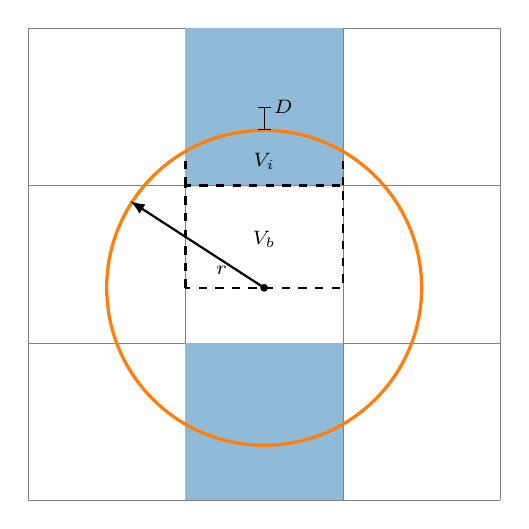
\begin{tikzpicture}[scale=1.0]
    \tikzstyle{every node}=[font=\scriptsize]
    \colorlet{lightBlue}{matplotlibBlue!50}
    
    \draw[step=2.0,gray,very thin] (0,0) grid (6,6);

    \fill[lightBlue] (2,4) rectangle ++(2,2);
    \fill[lightBlue] (2,0) rectangle ++(2,2);
    
    \begin{axis}
    [xmin=0,
    xmax=12.925,
    ymin=0,
    ymax=10,
    ticks=none,
    axis lines=none,
    clip=false,
    scale only axis
    ]
    \end{axis}
    
    % Particle
    \coordinate[] (xpj) at (3,2.7);
    \node[fill=black, circle, inner sep=1.0] at (xpj) {};
    \draw[matplotlibOrange,very thick] (xpj) circle (2.0);

    % Linear approximation
    % Dashed boxes
    \draw[thick, dashed] (2,2.7) rectangle (4,4);
    \draw[thick, dashed] (2,4)--(2,4.4);
    \draw[thick, dashed] (4,4)--(4,4.4);
    % Text
    \node[] at (3,3.3) {$V_b$\strut};
    \node[] at (3,4.3) {$V_i$\strut};

    % Radius arrow
    \draw[-latex, thick] (xpj) -- ++(-1.7,1.1) node[pos=0.2,left]{$r$};

    % D arrow
    \draw[black, |-|,  >={Latex[scale=0.75]}] (3,4.7) -- (3,5) node[right]{$D$};
\end{tikzpicture}

  \caption{
        The linear approximation yields the analytical solution for the blue cells. The particle is represented by the orange circle. Note that the grid is coarsened for better clarity.
    }\label{fig:linear_approximation}
\end{figure}
In \cref{fig:linear_approximation}, the overlap fraction $\epsilon$ between the upper blue lattice cell and the orange particle is computed as
\begin{equation}
  \epsilon=V_i=V_a-V_b=V_a-(D+r-1/2),
\end{equation}
where $V_a$ is the union of $V_i$ and $V_b$. $D$ is the distance from the cell center to the sphere surface (negative if the cell center lies inside the sphere). There is a cell-particle overlap if $\epsilon \in \interval[open left]{0}{1}$. We can reformulate this as
\begin{equation}
  \epsilon=V_a-(D+r-1/2)=-D+f(r),
\end{equation}
where $f(r)=V_a-r+1/2$ only depends on the particle radius $r$ and therefore is constant for each particle respectively.
$V_a$ is computed as
\begin{dmath}
  V_a=\int_{-1/2}^{1/2}\int_{-1/2}^{1/2} \sqrt{r^2-x^2-y^2} \text{d}x \text{d}y= (1/12-r^2)\tan^{-1} (\frac{\frac{1}{2}\sqrt{{r^2}-1/2}}{1/2-r^2})+\frac{1}{3}\sqrt{{r^2}-1/2}\\
  + (r^2- 1/12)\tan^{-1} (\frac{1/2}{\sqrt{{r^2}-1/2}})\\-\frac{4}{3}r^3\tan^{-1} (\frac{1/4}{r\sqrt{{r^2}-1/2}}).
\end{dmath}
This approximation yields accurate results also for arbitrary cell orientations and is more computationally efficient than contemporary techniques like sub-division sampling \citep[][]{jonesFastComputationAccurate2017}.

\section{Implementation}\label{implementation}
We implemented our hybrid coupled fluid-particle simulation within the massively parallel multiphysics framework \walberla~\citep[][]{bauerWaLBerlaBlockstructuredHighperformance2021a} (\url{https://www.walberla.net/}).\ \walberla~supports highly efficient and scalable \gls{lbm} simulations on both \glspl{cpu} and \glspl{gpu}~\citep[][]{holzerHighlyEfficientLattice2021}.
The MesaPD module~\citep[][]{eiblModularExtensibleSoftware2019} enables \walberla~to perform particle simulations on \glspl{cpu} using the \gls{dem}.
Large-scale simulations require the usage of numerous nodes of a supercomputer. Each node of a heterogeneous supercomputer typically consists of one or many \glspl{cpu} and \glspl{gpu}. Several \gls{cpu} cores belong to one \gls{gpu}, i.e., they have a direct connection. We divide the simulation domain into multiple blocks and exclusively assign each block to a \gls{gpu}. Figure~\ref{fig:domain_partitioning} illustrates the domain partitioning and the respective hardware assignment.
\begin{figure}
  \centering
  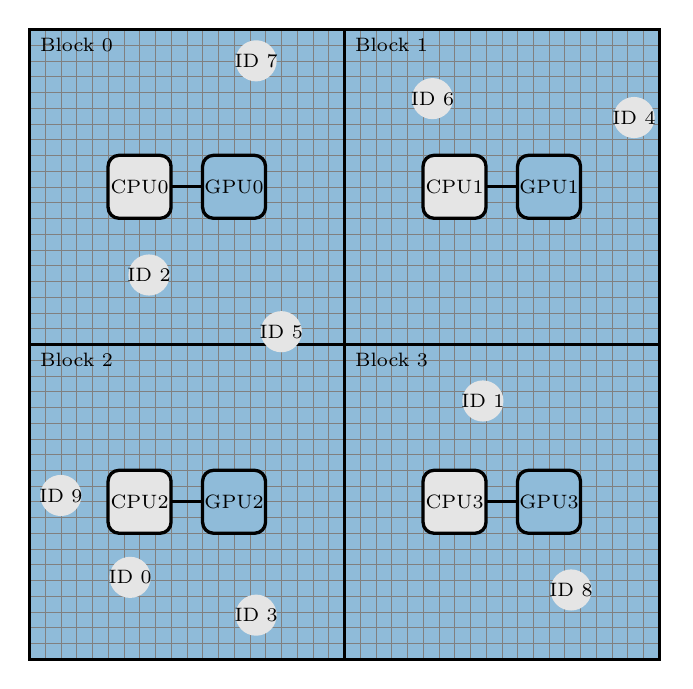
\begin{tikzpicture}[scale=0.8]
    \tikzstyle{every node}=[font=\scriptsize]

    \colorlet{blue}{matplotlibBlue!50}
    
    % Add domain
    \fill[blue] (0,0) rectangle (10.0,10.0);
    
    \draw[step=0.25,gray,very thin] (0,0) grid (10.0,10.0);
    \draw[black,very thick] (0,0) rectangle (5,5);
    \draw[black,very thick] (5,0) rectangle (10,5);
    \draw[black,very thick] (0,5) rectangle (5,10);
    \draw[black,very thick] (5,5) rectangle (10,10);

    \node[black] at (0.75,9.75) {Block 0};
    \node[black] at (5.75,9.75) {Block 1};
    \node[black] at (0.75,4.75) {Block 2};
    \node[black] at (5.75,4.75) {Block 3};

    % Add particles inside domain
    \draw[gray!20, fill=gray!20, very thick] (1.6,1.3) circle (0.3) node [black] {ID 0};
    \draw[gray!20, fill=gray!20, very thick] (7.2,4.1) circle (0.3) node [black] {ID 1};
    \draw[gray!20, fill=gray!20, very thick] (1.9,6.1) circle (0.3) node [black] {ID 2};
    \draw[gray!20, fill=gray!20, very thick] (3.6,0.7) circle (0.3) node [black] {ID 3};
    \draw[gray!20, fill=gray!20, very thick] (9.6,8.6) circle (0.3) node [black] {ID 4};
    \draw[gray!20, fill=gray!20, very thick] (4,5.2) circle (0.3) node [black] {ID 5};
    \draw[gray!20, fill=gray!20, very thick] (6.4,8.9) circle (0.3) node [black] {ID 6};
    \draw[gray!20, fill=gray!20, very thick] (3.6,9.5) circle (0.3) node [black] {ID 7};
    \draw[gray!20, fill=gray!20, very thick] (8.6,1.1) circle (0.3) node [black] {ID 8};
    \draw[gray!20, fill=gray!20, very thick] (0.5,2.6) circle (0.3) node [black] {ID 9};

    % Add hardware
    \draw[black, fill=gray!20, very thick, rounded corners] (1.25,7) rectangle (2.25,8) node [black, pos=.5] {CPU0};
    \draw[black, fill=blue, very thick, rounded corners] (2.75,7) rectangle (3.75,8) node [black, pos=.5] {GPU0};
    \draw[black, fill=gray!20, very thick, rounded corners] (6.25,7) rectangle (7.25,8) node [black, pos=.5] {CPU1};
    \draw[black, fill=blue, very thick, rounded corners] (7.75,7) rectangle (8.75,8)  node [black, pos=.5] {GPU1};
    \draw[black, fill=gray!20, very thick, rounded corners] (1.25,2) rectangle (2.25,3) node [black, pos=.5] {CPU2};
    \draw[black, fill=blue, very thick, rounded corners] (2.75,2) rectangle (3.75,3) node [black, pos=.5] {GPU2};
    \draw[black, fill=gray!20, very thick, rounded corners] (6.25,2) rectangle (7.25,3) node [black, pos=.5] {CPU3};
    \draw[black, fill=blue, very thick, rounded corners] (7.75,2) rectangle (8.75,3) node [black, pos=.5] {GPU3};

    \draw [black, very thick] (2.25,7.5) -- (2.75,7.5);
    \draw [black, very thick] (7.25,7.5) -- (7.75,7.5);
    \draw [black, very thick] (2.25,2.5) -- (2.75,2.5);
    \draw [black, very thick] (7.25,2.5) -- (7.75,2.5);
\end{tikzpicture}

  \caption{
        Partitioning of a 2D simulation domain into four blocks. The circles with ID 0 to ID 9 indicate the particles, and the blue cells are the fluid. One \gls{gpu}x for updating the fluid cells is assigned to each block x, and the corresponding \gls{cpu}x cores are responsible for the particle dynamics. \gls{cpu}x represents the \gls{cpu} cores having a direct connection/affinity to \gls{gpu}x. MPI rank x is assigned to \gls{cpu}x, distributes the particle computations among \gls{cpu}x using OpenMP, and uses \gls{gpu}x for the fluid dynamics.
    }\label{fig:domain_partitioning}
\end{figure}
We want to highlight that the particle simulation is not a standalone framework, but for the particles and the fluid that are physically close to each other (i.e., in the same block), one MPI process is responsible for both the particle and fluid dynamics and the \gls{cpu} and \gls{gpu} have a direct connection/affinity.
The \gls{cpu} cores belonging to the respective \gls{gpu} are responsible for updating the particles whose center of mass lies inside that block (local particles). In Figure~\ref{fig:domain_partitioning}, \gls{cpu}0 is responsible for the particles with ID 2, 5, and 7.
Additionally, particles can overlap with a given block whose center of mass lies in another block (ghost particles). In Figure~\ref{fig:domain_partitioning}, the particle with ID 5 is local for block 0 and ghost for block 2. This overlapping causes the need for communication between the \glspl{cpu}. The particle computations within a block are parallelized among the \gls{cpu} cores using OpenMP.~The communication between neighboring blocks is implemented using the CUDA-Aware Message Passing Interface. On clusters with multiple \glspl{gpu} sharing a node and NVLinks between the \glspl{gpu}, NVIDIA GPUDirect is used for direct GPU-GPU MPI communications between the \glspl{gpu} on the node.
\cref{fig:implementation} illustrates the different modules of the simulation, on which hardware they are running, the workflow, and the necessary communication steps. We will explain the figure in detail in the following sections. Generally speaking, the \gls{gpu} is responsible for all operations on fluid cells (i.e., the \gls{lbm} and the coupling), whereas the \gls{cpu}  performs all computations on particles. The associated data structures are consequently located in the respective memories (fluid cells in \gls{gpu} memory, particles in \gls{cpu} memory).
\begin{figure}
  \centering
  \section{Implementation}
\label{sec:impl}

At \company, we have deployed \sysname in our internal clusters to serve daily DL workloads.
The internal clusters consist of heterogeneous GPUs, including NVIDIA T4 GPU and NVIDIA A10 GPU.
Integrated with Kubernetes~\cite{k8s}, \sysname manages thousands of GPUs in each cluster and more than 20,000 GPUs in all.

\parabf{Service manager.}
For online workloads, we use the existing service manager at \company which deploys containers, discovers service, and autoscales horizontal pods.

\parabf{Global manager.}
We modify the Kubernetes scheduler to schedule offline workloads.
The workload profiler takes several dedicated GPUs, whose number is negligible to the total number of GPUs.
When a new offline workload comes, the workload profiler performs a few dry runs of the workload and utilizes the NVIDIA Data Center GPU Manager (DCGM) tools~\cite{dcgm} and NVIDIA Management Library (NVML)~\cite{nvml} libraries to collect GPU metrics.
We collect about 2,000 data for each GPU type to train the speed predictor.
The MLPs of the speed predictor have four layers with hidden size $64\times 64$.
The MLPs are trained with momentum SGD optimizer~\cite{ruder2016overview} in PyTorch v1.8.0~\cite{paszke2019pytorch} until they converge.
\sysname invokes the scheduler periodically to schedule all offline workloads.
When moving workloads, we record checkpoints of offline workloads and restart the workloads after transmitting the models and checkpoints.
As the datasets are usually colossal, we store the datasets in a remote file system and fetch data during the execution.
We implement the scheduler as a third-party plugin to the Kubernetes scheduler.


\parabf{Local executor.}
Each local executor executes online workloads according to the service manager and offline workloads according to the global manager.
DL workloads are executed in Docker containers with our customized components.
We add Best-Effort GPU DevicePlugin in Kubernetes and relevant control paths with Kubelet and \sysprobe for offline workloads.
To control SM percentage, we leverage the environment variable $CUDA\_MPS\_ACTIVE\_THREAD\_PERCENTAGE$ provided by MPS.
The GPU monitor collects resource metrics through DCGM~\cite{dcgm} and NVML~\cite{nvml} for NVIDIA GPU.
The \sysprobe updates the state machine with the collected resource metrics and empirically-set thresholds.
When the state is unhealthy, the \sysprobe will ask the NodeManager in Kubernetes to evict offline workloads.
\bytecuda intercepts nearly 800 CUDA driver APIs for GPU memory allocation and kernel launch.
The GPU memory quota of offline workloads is fixed to $40\%$ as Figure~\ref{fig:motiv_gpu_resource} reports that most online workloads use less than $60\%$ GPU memory.
We adopt the cpuset of Cgroup for CPU isolation.
For memory, \sysname will evict offline workloads if memory usage is higher than a threshold or the kernel swap daemon is busy for a long time.
The parameters to calculate GPU load in Equation~\ref{equ:gpu_load}$\&$\ref{equ:clock_factor} are empirically selected through trial-and-error.

  \caption{
        Flowchart of our hybrid \gls{cpu}-\gls{gpu} implementation from the perspective of a \gls{cpu} and \gls{gpu} responsible for the same block. The color coding indicates the communication types required within each step.
    }\label{fig:implementation}
\end{figure}

\subsection{Fluid dynamics and coupling on the GPU}
Performing an \gls{lbm} update step requires the communication of boundary cells between neighboring \glspl{gpu}. However, the first three kernels do not need neighboring information. Therefore, the communication is hidden behind those kernels by starting a non-blocking send before the particle mapping. A time step begins with the coupling from the particles to the fluid.

\subsubsection{Coupling from the particles to the fluid}
For the particle mapping, the \gls{gpu} has to check overlaps for all cell-particle combinations, even though there is no overlap for most cell-particle combinations. This check quickly becomes very computationally expensive. Therefore, we reduce the computational effort by dividing each block into $k$ sub-blocks in each dimension.
The \gls{cpu} inserts every particle into all sub-blocks that overlap with this particle, similar to the Linked Cell Method. Using sub-blocks allows the \gls{gpu} to consider only a tiny subset of particles when computing the overlaps for a particular grid cell, namely the particles overlapping with the sub-block the cell is located in.
Our coupled fluid-particle simulation requires the communication of various data. \cref{fig:compute_setup} gives an overview of the different types of communication from the perspective of a \gls{cpu} and \gls{gpu} responsible for the same block. We will explain the communication steps in the following.
For every particle $i$, the position $\boldsymbol{x}_{\text{p},i}$, radius $r_i$, and $f(r_i)$ (\cref{particle_mapping}) are transferred from the \gls{cpu} to the \gls{gpu} via the PCIe. In addition, the number of overlapping particles per sub-block and the corresponding particle IDs are transferred from the \gls{cpu} to the \gls{gpu}.
Then, the \gls{gpu} performs the particle mapping. For more details, see the description of the solid volume fraction computation (i.e., the particle mapping) in \cref{particle_mapping}.
In our simulation, a maximum of two particles can overlap with a given grid cell due to the geometrically resolved spherical particles and appropriate \gls{dem} parameters allowing only a small particle-particle penetration. Therefore, the grid that we use to store $B_i(\boldsymbol{x},t)$, can store two fraction values per grid cell.
Next, the linear and angular velocities $\boldsymbol{U}_{\text{p},i}$ and ${\boldsymbol{\Omega}}_{\text{p},i}$ of the particles must be synchronized between the \glspl{cpu} such that every \gls{cpu} has not only the correct velocities for its local particles but also for the ghost particles. Next, those velocities are transferred from the \gls{cpu} to the \gls{gpu} so that the \gls{gpu} can compute the velocities of the overlapping particles at the cell center for every cell (\cref{vel_at_cell_center}).
\begin{figure*}
  \centering
  %\resizebox{13cm}{!}{
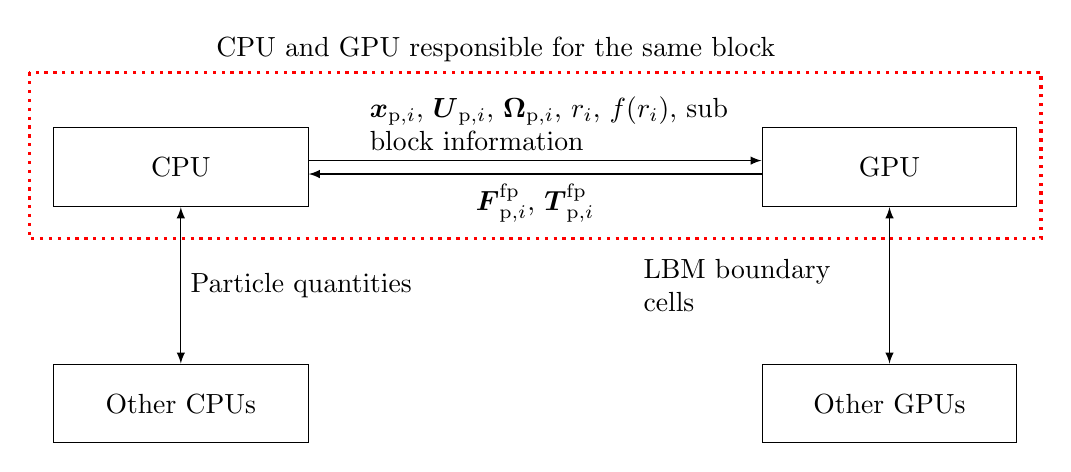
\begin{tikzpicture}[scale=1.0]
    % Nodes
    \node (cpu) [kernel] {CPU};
    \node (cpus) [kernel, below of=cpu, yshift=-2cm] {Other CPUs};
    \node (gpu) [kernel, right of=cpu, xshift=8cm] {GPU};
    \node (gpus) [kernel, below of=gpu, yshift=-2cm] {Other GPUs};

    % Frame
    \draw[red,very thick,dotted] ($(cpu.north west)+(-0.3,0.7)$)  rectangle ($(gpu.south east)+(0.3,-0.4)$);
    \node[] at (4,1.5) {CPU and GPU responsible for the same block};

    % Arrows
    \draw [-latex] ([yshift=-12pt]cpu.north east) -- node (nextStep) [above, text width=5cm, xshift=0.4cm] {$\boldsymbol{x}_{\text{p},i}$, $\boldsymbol{U}_{\text{p},i}$, ${\boldsymbol{\Omega}}_{\text{p},i}$, $r_i$, $f(r_i)$, sub block information} ([yshift=-12pt]gpu.north west);
    \draw [-latex] ([yshift=12pt] gpu.south west) -- node (nextStep) [below] {$\boldsymbol{F}_{\text{p},i}^{\text{fp}}$, $\boldsymbol{T}_{\text{p},i}^{\text{fp}}$} ([yshift=12pt] cpu.south east);
    \draw [latex-latex] (cpu) -- node (nextStep) [right, text width=3cm] {Particle quantities} (cpus); 
    \draw [latex-latex] (gpu) -- node (nextStep) [left, text width=3cm] {LBM boundary cells} (gpus);
\end{tikzpicture}
%}

  \caption{
        Overview of the different communication steps from the perspective of a \gls{cpu} and \gls{gpu} responsible for the same block
    }\label{fig:compute_setup}
\end{figure*}

\subsubsection{Fluid simulation}\label{fluid_simulation}
Next, the \gls{psm} inner kernel is performed. The term `inner' indicates that this kernel updates all cells except the outermost layer of cells. Skipping the outermost layer ensures that this routine can be called without waiting for the previously started \gls{gpu}-\gls{gpu} communication to finish.
The \gls{psm} kernel creates the highest workload of the entire simulation. It is, therefore, performance-critical. We use the code generation framework lbmpy~\citep[][]{bauerLbmpyAutomaticCode2021, hennigAdvancedAutomaticCode2023} to obtain highly efficient and scalable \gls{lbm} CUDA kernels.\ lbmpy allows the formulation of arbitrary \gls{lbm} methods (such as the \gls{psm}) as a symbolic representation and generates optimized and parallel compute kernels. We integrate those generated compute kernels within the simulation in \walberla.
Next, we wait for the non-blocking \gls{gpu}-\gls{gpu} communication started at the beginning of the time step to finish. Depending on the available hardware, this may return instantly if the previous computations completely hide the communication.
The next step is the \gls{lbm} boundary handling, which enforces boundary conditions to the fluid simulation by correctly updating the fluid cells at the domain's boundary.
Since the neighboring values are now available, we then update the outermost layer of cells in the \gls{psm} outer kernel.
The last step on the \gls{gpu} is the coupling from the fluid to the particles.

\subsubsection{Coupling from the fluid to the particles}
Finally, the \gls{gpu} reduces the forces and torques exerted by the fluid on the particles $\boldsymbol{F}_{\text{p},i}^{\text{fp}}$ and $\boldsymbol{T}_{\text{p},i}^{\text{fp}}$ (\cref{hydrodynamic_force,hydrodynamic_torque}).
Then, $\boldsymbol{F}_{\text{p},i}^{\text{fp}}$ and $\boldsymbol{T}_{\text{p},i}^{\text{fp}}$ are transfered from the \gls{gpu} to the \gls{cpu} to be available for the upcoming \gls{dem} simulation on the \gls{cpu}. 
A single particle may overlap with cells located on multiple blocks. Thus, multiple \glspl{gpu} may have computed $\boldsymbol{F}_{\text{p},i}^{\text{fp}}$ and $\boldsymbol{T}_{\text{p},i}^{\text{fp}}$ for the same particle $i$. Therefore, the corresponding \glspl{cpu} have to reduce these force and torque contributions exerted by the coupling on the particles into a single variable (\gls{cpu}-\gls{cpu} communication).
The time loop continues with the particle dynamics on the \gls{cpu}.

\subsection{Particle dynamics on the CPU}\label{particle_dynamics}
The first step of the \gls{pd} simulation on the \gls{cpu} is the pre-force integration of the velocities to update the particle positions (\cref{pre_force_integration}). The latter particle movement requires synchronization between the \glspl{cpu} to account for the position update, which potentially moves particles from one block to another, making other \glspl{cpu} responsible for the particles. Computing particle-particle interactions by iterating over all particle pairs can quickly become very expensive due to its $O(n^2)$ complexity. Therefore, we insert the particles into linked cells such that iterating over the particle pairs is limited to neighboring linked cells. The linked cell size limits the maximum distance for which correct particle-particle interactions can be ensured (collision, lubrication correction). The linked cells have a size of 1.01 times the particle diameter, which is close to the smallest size that still leads to a correct collision detection.
Next, the lubrication correction routine is applied to all particle pairs with particles close to each other but not yet in contact (\cref{lubrication_correction}).
The particle-particle interactions are modeled using the \gls{dem} collision kernel (linear spring dashpot), which exerts forces and torques on overlapping particles.
The collision kernel needs history information from the previous time step, i.e., the accumulated tangential motion between the two colliding particles (\cref{history_information}). Since different processes may have handled the previous collisions, reducing the collision histories between the \glspl{cpu} is necessary, i.e., collecting all collision histories for a given particle in one process.
Then, the hydrodynamic forces and torques exerted by the fluid on the particles and the gravitational force are added to the total force.
Since different processes may have added forces and torques to a given particle, those contributions have to be collected in one process (another \gls{cpu}-\gls{cpu} communication).
Then, the post-integration is applied to update the particle velocities (\cref{post_force_integration}). Communication can be omitted here because the velocities are unused until the subsequent communication in the upcoming sub-cycle. 
Typically, $j$ particle sub-cycles are performed per time step since the \gls{dem} requires a finer resolution in time than the \gls{lbm} for an accurate contact representation~\citep[][]{rettingerEfficientFourwayCoupled2022}.
After completing $j$ sub-cycles, the next time step starts with the fluid dynamics on the \gls{gpu}.\newline
Running the fluid dynamics and coupling on the \gls{gpu} first and the particle dynamics on the \gls{cpu} second seems to be a promising candidate for overlapping the \gls{cpu} and \gls{gpu} computations to gain some performance improvements. Therefore, we elaborate on this possibility in the remainder of this section.
The following will refer to the different simulation modules as they are named in \cref{fig:implementation}.\newline
Under the condition that the numerical error must not increase, only some parts of the \gls{cpu} and \gls{gpu} computations can overlap, others cannot due to the dependencies of the two-way coupling. 
There are two ways of overlapping the \gls{cpu} and \gls{gpu} parts: within a time step or between subsequent time steps.
Only the post-force integration step of the particle simulation on the \gls{cpu} in time step $n$ depends on the reduction of the hydrodynamic forces on the \gls{gpu} in time step $n$, and therefore, the steps from pre-force integration to the application of external forces can, in principle, be overlap with the \gls{gpu} part.
The particle mapping on the \gls{gpu} at the beginning of time step $n+1$ requires the updated particle positions of the pre-force integration in time step $n$. Therefore, the steps from inserting the particles into linked cells until the post-force integration in time step $n$ can, in principle, overlap with the particle mapping on the \gls{gpu} in time step $n+1$.
However, the particle simulation typically consists of several sub-cycles (i.e., the \gls{cpu} part in \cref{fig:implementation} is executed several times per time step), and only the respective parts of the first and last sub-cycle can be overlapped. Therefore, the maximum achievable speedup due to overlapping depends on the number of sub-cycles. In accordance with the literature~\citep[][]{rettingerEfficientFourwayCoupled2022}, we use ten sub-cycles, which could potentially decrease the run time of the particle simulation on the \gls{cpu} by 20\% if the first and last sub-cycles could be entirely overlapped. However, this is an optimistic assumption because the interruption of the consecutive particle sub-cycles by the overlapping might negatively affect the possibility of caching particle data between consecutive sub-cycles.\newline
If one disregards the requirement that numerical error must not increase, one could use results from previous time steps, allowing both the fluid simulation on the \gls{gpu} and the particle simulation on the \gls{cpu} to run entirely in parallel. This might result in acceptable minor errors for systems with negligible particle movements, but this is not generally applicable and would require a detailed error analysis.

\section{Performance analysis}\label{performance}
We use the Juwels Booster cluster for the performance measurements. Each GPGPU node consists of four Nvidia A100 40 GB, two AMD EPYC 7402 processors (24 cores per chip), and eight NUMA domains. Thus, six cores belong to one NUMA domain. The following will refer to a \gls{gpu} and an associated NUMA domain with its six cores as a CPU-GPU pair. All \gls{gpu}s within a node are connected via NVLinks, allowing direct \gls{gpu}-\gls{gpu} communications. A scaling benchmark (i.e., a 1:1 read/write ratio) yields a memory bandwidth of about 1400 GB/s for the A100 40 GB~\cite{ernstAnalyticalPerformanceEstimation2023}. % https://github.com/te42kyfo/gpu-benches/blob/master/gpu-stream/a100_40.txt
We use 20 cells per diameter to geometrically resolve the particles~\cite{rettingerRheologyMobileSediment2022, rettingerEfficientFourwayCoupled2022, biegertCollisionModelGrainresolving2017, costaCollisionModelFully2015}.
The upcoming sections first introduce the computational properties of the simulated cases, followed by their performance results.

\subsection{Simulation setups}\label{setups}
We study the performance of our hybrid coupled fluid-particle implementation using a fluidized bed simulation. We compare two cases: the dilute case and the dense case. They exhibit different characteristics regarding the number of particles per volume and the number of particle-particle interactions. We choose these two cases to investigate how different particle workloads on the \gls{cpu}s influence the overall performance of the hybrid \gls{cpu}-\gls{gpu} implementation.
We use ten particle sub-cycles (see \cref{implementation}) per time step.
We discretize the simulated domain using $500 \times 200 \times 800 = 80 \times 10^6$ fluid cells. The inflow \gls{bc} on the bottom and pressure (outflow) \gls{bc} on top of the domain govern the fluid dynamics. The remaining four boundaries are no-slip conditions ensuring a zero fluid velocity. The particle Reynolds number is $1.0$, the Galileo number is around $8.9$, the gravitational acceleration is $9.81\ \text{m}/\text{s}^2$, and the particle fluid density ratio is $1.1$.
Planes surrounding the domain prevent the particles from leaving the domain.
The dilute case contains 627 particles. \cref{fig:fluidized_bed} (left) illustrates the dilute setup.
Due to the low particle concentration, the effort for computing the particle-particle interactions (collisions and lubrication corrections) is low in the dilute case. 
The dense case is generally the same setup as the dilute case, except that the particle concentration is significantly higher (see \cref{fig:fluidized_bed} on the right), resulting in 8073 particles, almost a 13-fold increase compared to the dilute case.

\begin{figure}
  \centering
  \includegraphics[scale=0.5, height=10cm]{figures/dilute_case.png}
  \includegraphics[scale=0.5, height=10cm, trim=0 0.65cm 0 -0.65cm]{figures/dense_case.png}
  \caption{Visualization of the fluidized bed setup running on one CPU-GPU pair. Dilute case on the left, dense case on the right. For the fluid field, only a two-dimensional slice is visualized.}\label{fig:fluidized_bed}
\end{figure}

\subsection{Performance results}
In this section, we present and analyze the performance results. We first look into the scaling of the \gls{pd} on multiple \gls{cpu} cores to assess our initial assumption that the particle simulation part of such a coupled simulation would not benefit from a GPU parallelization.
Next, we look at the individual run times of the different simulation components to understand the bottlenecks.
Furthermore, we present a weak scaling benchmark for both cases up to 1024 \gls{cpu}-\gls{gpu} pairs.
Finally, we demonstrate the acceleration potential of hybrid implementations by comparing it to a large-scale \gls{cpu}-only simulation from the literature.
For all results, we average over 500 time steps.
In the following, we will refer to the performance criteria formulated in the introduction.

\subsubsection{Particle scaling on the CPU}
% Description
Using OpenMP with static scheduling, we parallelize the \gls{pd} simulation on the \gls{cpu}.\@ Per-particle computations (e.g., adding gravitational forces) are parallelized among the particles, and particle-particle interactions are parallelized among the linked cells in one dimension. We use multiple cores of a single \gls{cpu} and measure the run time of the \gls{pd} simulation. The parallel efficiency $E_n$ is defined based on the serial run time $t_{\text{s}}$ and the run time using $n$ cores in parallel $t_{\text{p}}(n)$:

\begin{equation}
  E_n=\frac{t_s}{t_{\text{p}}(n) \cdot n}.
\end{equation}

\noindent
For a perfectly linear scaling code, i.e., $t_{\text{p}}(n)=t_s/n$, the maximum achievable parallel efficiency $E_{\max}$ is 1 $\forall n$. For a non-scaling code, i.e., $t_{\text{p}}(n)=t_{\text{s}}\ \forall n$, the minimum achievable parallel efficiency $E_{\min}$ is $1/n$.\ \cref{fig:particle_scaling} reports the parallel efficiency of the \gls{pd} simulation for both cases for up to six cores, i.e., the size of a NUMA domain. We do not use more cores than available in a NUMA domain since the \gls{pd} implementation is not NUMA-aware. % ist das so und warum wäre es ein Problem das NUMA-aware zu implementieren?

\begin{figure}
  \centering
  \begin{tikzpicture}
    \begin{axis}[
        xlabel=Threads,
        ylabel=Parallel Efficiency $E$,
        legend style={at={(0.98,0.65)},anchor=east},
        legend cell align={left},
        width=0.9*\textwidth,
        height=0.4*\textheight,
        grid
        ]
  
    \draw [ultra thick, matplotlibGreen!50] (1,1) -- (6,1);
    \addlegendimage{matplotlibGreen}
    \addlegendentry{$E_{\max}$}
  
    \addplot[mark=*, mark size=3pt, very thick, matplotlibBlue] plot coordinates {
      (1,1.0)
      (2,0.7581699346405228)
      (3,0.6137566137566137)
      (4,0.5132743362831859)
      (5,0.46399999999999997)
      (6,0.46586345381526106)
    };
    \addlegendentry{Dilute case}
  
    \addplot[mark=diamond*, mark size=3pt, very thick, matplotlibOrange] plot coordinates {
      (1,1.0)
      (2,0.7014660151043981)
      (3,0.6199450333725952)
      (4,0.5231941683233929)
      (5,0.48103579588728096)
      (6,0.4492815478730972)
    };
    \addlegendentry{Dense case}
  
    \addplot[domain=1:6, ultra thick, matplotlibRed!50]{1/x};
    \addlegendentry{$E_{\min}$}
  
    \end{axis}
\end{tikzpicture}

  \caption{Parallel efficiency inside a NUMA domain for both cases. The perfect scaling (Best) and non-scaling (Worst) form the upper and lower bound. }\label{fig:particle_scaling}
\end{figure}

\noindent
% Observations
We observe a similar pattern regarding the parallel efficiency in both the dilute and the dense case. Both show a decrease down to around 45\% for six cores.\newline
% Interpretation
A parallel efficiency of about 45\% when using a comparatively small number of six cores is a poor scaling result. We expect this performance for several reasons. First, the \gls{pd} simulation consists of ten subsequent sub-cycles per time step, each containing several consecutive tasks (see \cref{fig:implementation}). Each task consists of an OpenMP parallel loop with an implicit OpenMP barrier at the end, causing idle threads to wait for all threads to end the loop. Second, modifying the force and torque of a particle must be enclosed with an atomic region to avoid race conditions, which harms the parallel efficiency, but is a central task and thus required in several \gls{pd} routines. Third, the workload (for the \gls{dem} and lubrication routine) per particle can differ significantly depending on the particle's location inside the domain. The latter aspects hold for the dense and the dilute case, explaining the poor parallel efficiency in both cases.
The poor parallel efficiency of the particle methodology supports our initial assumption that the particle simulation part would not benefit from a \gls{gpu} parallelization in the context of geometrically resolved coupled simulations.

\subsubsection{Run times of different simulation components}
% Description / Reference
We investigate the run times of the different simulation components to analyze the penalty introduced by the hybrid implementation, i.e., the \gls{cpu}-\gls{gpu} communication, assess the \gls{gpu} performance, and detect the overall bottlenecks. To evaluate the performance of the \gls{psm} kernel on the \gls{gpu}, we build a roofline model~\cite{hagerIntroductionHighPerformance2010} for an \gls{lbm} kernel. As this kernel is memory bound, we determine the maximal possible performance for the given kernel and hardware when fully utilizing the memory bandwidth (i.e., the performance lightspeed estimation). The \gls{psm} kernel comprises the \gls{lbm} kernel plus additional memory transfers depending on the number of overlapping particles. As this number differs from cell to cell, the \gls{psm} roofline model is not straightforward. Therefore, we use the \gls{lbm} model, keeping in mind that this is a too-optimistic performance lightspeed estimation.
Since we use the D3Q19 lattice model, we read and write 19 \gls{pdfs} per cell and time step.
This results in 19 reads and 19 writes (double-precision), i.e., 304 bytes to update one lattice cell~\cite{feichtingerPerformanceModelingAnalysis2015}. The domain consists of $8e7$ fluid cells. This results in the following minimal run time according to the roofline model:

\begin{equation}
  T_\min = \frac{304 \ \text{B/cell} \cdot 8e7 \ \text{cells/time step}}{1400 \ \text{GB/s}} = 17.4 \ \text{ms/time step}.
\end{equation}

\noindent
We divide the total run time into the following components: the \gls{psm} kernel (PSM), the \gls{cpu}-\gls{gpu} communication (comm), the particle mapping (mapping), setting the particle velocities (setU), reducing the hydrodynamic forces $\boldsymbol{F}_{\text{p},i}^{\text{fp}}$ and torques $\boldsymbol{T}_{\text{p},i}^{\text{fp}}$ on the particles (redF), computing the \gls{pd} and finally the remaining tasks (other), e.g., the \gls{lbm} boundary handling.\ \cref{fig:runtimesa100} reports the run times per time step for these components using a single \gls{cpu}-\gls{gpu} pair.

\begin{figure}
  \centering
  \pgfplotsset{/pgfplots/horizontal line legend/.style={legend image code/.code={\draw[very thick] (0cm,0cm)-- (.35cm,0cm);},},}

\begin{tikzpicture}
    \begin{axis} [ybar,
    ylabel=Time per time step / ms,
    symbolic x coords={PSM, comm, mapping, setU, redF, PD, other},
    xtick={PSM, comm, mapping, setU, redF, PD, other},
    xticklabel style={text height=2ex},
    legend style={at={(0.55,0.8)},anchor=east},
    legend cell align={left},
    grid, width=0.9*\textwidth, height=0.4*\textheight]
    \addplot [draw=matplotlibBlue,fill=matplotlibBlue!50, postaction={pattern=north east lines}, pattern color=black] coordinates {
        (PSM,24.78315357)
        (redF,4.912856478)
        (mapping,3.210133870259481)
        (setU,1.485454394)
        (PD,1.8600000000000003)
        (other,3.5557743957405172)
        (comm,0.10502729200000001)
    };
    \addplot [draw=matplotlibOrange,fill=matplotlibOrange!50, postaction={pattern=north east lines}, pattern color=black] coordinates {
        (PSM,31.901119082)
        (redF,18.391524202)
        (mapping,5.8220524171656685)
        (setU,2.792142046)
        (PD,41.96)
        (other,7.24992760483435)
        (comm,0.381234648)
        
    };
    \addplot[black,horizontal line legend,sharp plot,update limits=false,very thick] coordinates { ([normalized]-0.4,17.4) ([normalized]0.4,17.4) };
    \legend{Dilute case, Dense case, LBM roofline $T_\min$}
    \end{axis}
\end{tikzpicture}

  \caption{Individual run times of the different simulation components on a \gls{cpu}-\gls{gpu} pair.}\label{fig:runtimesa100}
\end{figure}

\noindent
% Observations
In the dilute case, the \gls{psm} kernel needs about 42\% more time per time step than the \gls{lbm} lightspeed estimation, and the dense case 83\% more time. The \gls{cpu}-\gls{gpu} communication is negligible for both cases. All components take longer in the dense case than in the dilute case. While in the dilute case, the \gls{psm} kernel accounts for the majority of the run time, the \gls{pd} simulation needs more time than the \gls{psm} kernel in the dense case. Still, most of the run time is spent on \gls{gpu} routines in the dense case.\newline
% Interpretation
The penalty introduced by the hybrid implementation is negligible because we only transfer a small amount of double-precision values per particle but no fluid cells. The penalty, therefore, shows that a hybrid parallelization with the presented technique is a viable approach, and the first criterion is met. The performance of the \gls{psm} kernel is close to utilizing the total memory bandwidth of the A100, especially considering that the roofline model does not consider the memory traffic due to the solid part of the \gls{psm} kernel. Therefore, the second criterion is met. There is a significant performance gain for the \gls{psm} kernel on the \gls{gpu} compared to a \gls{cpu}-only implementation since the \gls{psm} kernel is utilizing almost the entire memory bandwidth, which is typically way lower on \gls{cpu}s.
Even in the dense case, the \gls{gpu} run time accounts for most of the total time because the fluid workload is much higher than the particle workload. Therefore, the third criterion is met.

\subsubsection{Weak scaling}
% Description
When increasing the simulation domain further to simulate physically relevant scenarios, using a single \gls{cpu}-\gls{gpu} pair is often insufficient. Instead, multiple pairs or even multiple nodes of a supercomputer have to be used. Therefore, a satisfactory weak scaling is inevitable. For weak scaling, the problem size is increased with an increasing number of \gls{cpu}-\gls{gpu} pairs, keeping the workload per \gls{cpu}-\gls{gpu} pair constant. When having a perfect weak scaling, the performance per \gls{cpu}-\gls{gpu} pair stays constant, independent of the number of \gls{cpu}-\gls{gpu} pairs used. Performance is work over time. In the context of \gls{lbm}, MLUPs is a standard performance metric for weak scaling, meaning how many mega lattice cell updates the hardware performs per second. 
We use the total run time for computing the MLUPs, containing both the \gls{cpu} (particles) and the \gls{gpu} (fluid, coupling) time. We have conducted a few benchmarking runs and will use the best sample in the following weak-scaling plots.
We start with a single \gls{cpu}-\gls{gpu} pair and a single domain block as described in \cref{setups}. We then double the number of \gls{cpu}-\gls{gpu} pairs several times until we reach 1024. At the same time, we double the domain blocks/size alternately in each direction: $2\times 1 \times 1$ blocks (two \gls{gpu}s), $2\times 2 \times 1$ blocks (four \gls{gpu}s), $2\times 2 \times 2$ (eight \gls{gpu}s), etc.\ \cref{fig:weak_scaling} reports the weak scaling for both cases. To the best of our knowledge, this is the most extensive weak scaling of a hybrid fluid-particle implementation presented in the literature.

\begin{figure}
  \centering
  \begin{tikzpicture}
    \begin{semilogxaxis}[
        xlabel=CPU-GPU pairs,
        ylabel=MLUPs per pair,
        log basis x={2},
        xmin=0.75,
        xmax=1536,
        ymin=0,
        %legend style={at={(1.35,0.5)},anchor=east},
        legend cell align={left},
        width=0.9*\textwidth,
        height=0.4*\textheight,
        grid
        ]
    \addplot[mark=*, mark size=3pt, very thick, matplotlibBlue] plot coordinates {
      (1,2027.3)
      (2,1963.23)
      (4,1814.74)
      (8,1756.03)
      (16,1712.99)
      (32,1599.67)
      (64,1537.87)
      (128,1525.81)
      (256,1493.45)
      (512,1481.59)
      (1024,1435.99)
    };
    \addplot[mark=diamond*, mark size=3pt, very thick, matplotlibOrange] plot coordinates {
      (1,706.613)
      (2,634.843)
      (4,568.501)
      (8,549.758)
      (16,519.1)
      (32,470.161)
      (64,476.227)
      (128,436.286)
      (256,377.213)
      (512,414.443)
      (1024,377.581)
    };
    \addlegendentry{Dilute case}
    \addlegendentry{Dense case}
    \end{semilogxaxis}
\end{tikzpicture}

  \caption{Weak scaling performance for both cases up to 1024 \gls{cpu}-\gls{gpu} pairs.}\label{fig:weak_scaling}
\end{figure}

\noindent
% Observations
We observe a roughly three times higher performance for the dilute case than for the dense case. Both cases show a parallel efficiency decrease particularly strong in the beginning. The parallel efficiency is 71\% in the dilute case and 53\% in the dense case when using 1024 \gls{cpu}-\gls{gpu} pairs, which corresponds to a domain size of $8000 \times 1600 \times 6400 = 8.192 \times 10^{10}$ fluid cells. A similar scaling behavior has been observed in the literature both for other hybrid~\cite{ kotsalosDigitalBloodMassively2021} and \gls{cpu}-only fluid-particle implementations~\cite{rettingerFullyResolvedSimulations2017}.\newline
% Description
Interpreting the overall weak scaling behavior requires an in-depth analysis of the scaling of the different simulation components. When using a single \gls{cpu}-\gls{gpu} pair, the dominating routines are the \gls{pd}, the \gls{psm} kernel, and the coupling (i.e., particle mapping, setting the particle velocities and reducing the hydrodynamic forces $\boldsymbol{F}_{\text{p},i}^{\text{fp}}$ and torques $\boldsymbol{T}_{\text{p},i}^{\text{fp}}$
on the particles). Additionally, we must now consider the communication (comm) overhead that arises from using multiple \gls{cpu}-\gls{gpu} pairs. On the one hand, this is the \gls{pd} communication (\gls{cpu}-\gls{cpu} communication), on the other hand, the PSM communication (\gls{gpu}-\gls{gpu} communication). \cref{fig:weak_scaling_routines_dilute} and \cref{fig:weak_scaling_routines_dense} show the weak scaling behavior of the dominating simulation components for both cases. The communication numbers cover the communications themselves, but also load imbalances between two communication.

\begin{figure}
  \centering
  \input{plots/weak_scaling_components_dilute.tex}
  \caption{Weak scaling performance of the dominating components for the dilute case up to 1024 \gls{cpu}-\gls{gpu} pairs.}\label{fig:weak_scaling_routines_dilute}
\end{figure}

\begin{figure}
  \centering
  \input{plots/weak_scaling_components_dense.tex}
  \caption{Weak scaling performance of the dominating components for the dense case up to 1024 \gls{cpu}-\gls{gpu} pairs.}\label{fig:weak_scaling_routines_dense}
\end{figure}

\noindent
% Observations
The different components show similar qualitative scaling behavior when comparing the two cases. The \gls{psm} kernel scales quite well in both cases. The corresponding \gls{gpu}-\gls{gpu} communication (\gls{psm} comm) is negligible. The \gls{pd} run time increases initially and then shows saturation. The \gls{cpu}-\gls{cpu} communication (\gls{pd} comm) increases drastically, overtaking the run time of the \gls{psm} kernel and the coupling in the dense case. The \gls{pd} and the corresponding communication are more relevant for the overall scaling in the dense case than in the dilute case. The coupling scales similarly to the \gls{pd}.\newline
% Interpretation
The \gls{psm} workload per \gls{gpu} stays constant in the weak scaling explaining the nearly perfect scaling.
Since we are hiding the \gls{psm} communication (see \cref{implementation}), we expect it to be negligible.
We expect the \gls{pd} and the coupling run time to increase initially because the number of neighboring blocks increases. More neighboring blocks lead to more ghost particles per block, resulting in a higher workload. This effect fades out when blocks have neighbors in all directions resulting in an almost linear scaling from this point on. This phenomenon has been reported in the literature~\cite{rettingerFullyResolvedSimulations2017}.
The methodology requires ten particle sub-cycles per time step and three communications per sub-cycle for a physically accurate simulation. Additionally, the simulation requires two \gls{cpu}-\gls{cpu} communications per time step apart from the sub-cycles (see \cref{fig:implementation}). We have 32 \gls{cpu}-\gls{cpu} communications per time step, which cannot be hidden behind other routines. It is the dominating factor for the decrease of the overall weak scaling performance in both cases. We assume this is due to these frequent synchronizations between the processes and the high pressure on the network.
Reducing the collision history is part of \gls{pd} comm, which includes swapping old and new contact information. Since this swap is also necessary without using multiple \gls{cpu}-\gls{gpu} pairs, \gls{pd} comm is bigger zero even when using a single \gls{cpu}-\gls{gpu} pair.
Overall, we observe a weak scaling performance that justifies using multiple supercomputer nodes. Therefore, the fourth criterion is met.

\subsubsection{Potential speedup of hybrid implementations}
We expect that the speedup of the hybrid implementation compared to a \gls{cpu}-only code $S_{\text{hyb}}$ can be estimated as

\begin{equation}
  S_{\text{hyb}}  \approx \frac{1}{1+ frac_{\text{acc}} \cdot (\frac{BW_{\text{CPU}}}{BW_{\text{GPU}}}-1)},
  \label{speedup}
\end{equation}

\noindent
where $BW_{\text{CPU}}$ and $BW_{\text{GPU}}$ are the \gls{cpu} and \gls{gpu} memory bandwidths. $frac_{\text{acc}}$ is the \gls{cpu}-only run time fraction of the component accelerated by the hybrid implementation. In our case, this is the \gls{psm} and the coupling. We assume $frac_{\text{acc}}$ is memory bound.
We compare our hybrid performance results with one of the largest \gls{cpu}-only simulations of polydisperse sediment beds~\cite{rettingerRheologyMobileSediment2022}.
The authors conducted the latter simulation on 320 Intel Xeon Platinum 8174 \gls{cpu}s. In total, they computed $2.25\cdot 10^{15}$ lattice cell updates in 48 hours, which leads to a performance of around 41 MLUPs per \gls{cpu} vs. 377 MLUPs per \gls{cpu}-\gls{gpu} pair in the dense case when using 1024 \gls{gpu}s. The latter numbers result in a measured speedup of around 9.2. 
For the Intel Xeon Platinum 8174, we measured a memory bandwidth $BW_{\text{CPU}}$ of 70 GB/s.
The estimated speedup based on \cref{speedup} is around 10.3 (assuming $frac_{\text{acc}}=0.95$ and $BW_{\text{GPU}}=1400\ \text{GB/s}$) which is similar to the measured speedup. The latter computation is only a rough estimate since it ignores effects due to different \gls{cpu}s, networks, physical setups, etc.

\section{Implications and lessons learned}\label{implications}
As a lesson learned, we discovered that the relatively small data transfers between \gls{cpu} and \gls{gpu} can become negligible for coupled applications exhibiting a significant imbalance of the data exchange between the coupled modules and the computations inside the modules in favor of the computations, making hybrid coupling a feasible approach.
This is particularly true for the application used in this work, as only the several orders of magnitude smaller particle data need to be exchanged, not the entire fluid field processed by the \gls{gpu}. As a result, only 0.35\% of the total run time is devoted to \gls{cpu}-\gls{gpu} communication in the dense case.
These findings can also be applied to other applications that exhibit this desired imbalance between computation data size and data transfer between the coupled modules. Other coupled applications, such as a huge flow field around complex deformable geometries like the deformation of blood cells in cellular blood flow, which is referenced in \cref{introduction}, can also exhibit this imbalance. Since the surface data acts as a boundary condition for the deformation simulation, just this surface data needs to be exchanged between the fluid and solid phases.
\change{Approaches with a high ratio of data exchange to computations} (i.e., exchange entire fields between \gls{cpu} and \gls{gpu} in each time step) have been found in the literature to perform undesired on previous architectures, this may change in the future due to new hardware developments.
High bandwidth memory transfer between \gls{cpu} and \gls{gpu} main memory is the trend of architectures like the NVIDIA GH200 Grace Hopper, which makes hybrid implementations promising for more applications (even up to transferring the entire \gls{gpu} data in every time step) and should be further studied in the future.\newline
The advantages of code generation (\cref{fluid_simulation}) are the subject of another lesson learned. We discovered that code generation adds an extra overhead during the implementation stage, which is only beneficial in a framework with long-term support if one depends on highly optimized similar codes, portability to other architectures, and a certain form of expandable, sustainable approach. 
However, because code generation is used, the code functions flawlessly with different \gls{lbm} variations on other modern \gls{gpu} architectures, such as the AMD MI250X, which uses the HIP API, as well as on consumer \glspl{gpu}. Subsequent work will encompass a systematic performance comparison.

\section{Conclusion}\label{conclusion}
% Restate problem
On heterogeneous systems, it is pragmatic and, therefore, attractive to use a hybrid parallelization, i.e., different simulation modules running on different hardware.
However, hybrid implementations increase the complexity of achieving good performance and scalability, especially on large-scale systems.
% Repeat what has been done
In this paper, we have examined a hybrid coupled fluid-particle simulation with geometrically resolved particles. We use \glspl{gpu} for the fluid dynamics, whereas the particle simulation runs on the \glspl{cpu}.
% Summarize arguments and findings
We have reported and studied the performance of this approach for two cases of a fluidized bed simulation that differ in terms of the number of particles per volume.
The overhead introduced by the hybrid implementation (i.e., \gls{cpu}-\gls{gpu} communication) is negligible because we are transferring only a small amount of data per particle but no fluid cells.
The performance of the fluid simulation is close to utilizing the full memory bandwidth of the A100, implying that using the \gls{gpu} is a good choice for the fluid simulation.
In both cases, the \gls{gpu} routines take most of the run time.
In a weak scaling benchmark, the hybrid fluid-particle implementation reaches a parallel efficiency of 71\% in the dilute case and 53\% in the dense case when using 1024 \gls{cpu}-\gls{gpu} pairs.
The current \gls{pd} methodology requires 32 \gls{cpu}-\gls{cpu} communication steps per time step, which is the driving force for the decrease of the overall parallel efficiency. Our results are limited insofar as different numbers of particle sub-cycles, fluid cells per diameter, etc., will result in different performance results.
% Key takeaways from the paper
We have formulated four criteria that a hybrid implementation must meet to be suitable for the responsible use of heterogeneous supercomputers.
The performance results have shown that our hybrid implementation fulfills all criteria, making it suitable for large-scale simulations on heterogeneous supercomputers.
% Future work / Outlook
In the future, we plan to investigate the particle communication steps in more detail regarding the bottleneck and optimization possibilities. We are employing sub-cycles to increase stability for stiff systems. Using other integrators may permit longer time steps and thus less communication due to sub-cycles. We have shown the acceleration potential of hybrid implementations. Therefore, we plan to run coupled fluid-particle simulations of even larger scenarios to better analyze, among others, the physical phenomena of erosion in sediment beds.


\section*{Acknowledgements}
The authors gratefully acknowledge the Gauss Centre for Supercomputing e.V. (\url{www.gauss-centre.eu}) for funding this project by providing computing time on the GCS Supercomputer JUWELS at Jülich Supercomputing Centre (JSC).\newline
The authors gratefully acknowledge the scientific support and HPC resources provided by the Erlangen National High Performance Computing Center (NHR@FAU) of the Friedrich-Alexander-Universität Erlangen-Nürnberg (FAU). The hardware is funded by the German Research Foundation (DFG).

\section*{Declaration of competing interest}
The Authors declare that there is no conflict of interest.

\section*{Funding}
The authors disclosed receipt of the following financial support for the research, authorship, and/or publication of this article: The authors thank the Deutsche Forschungsgemeinschaft (DFG, German Research
Foundation) for funding the project 433735254. The DFG had no direct involvement in this paper; and this work has received funding from the European High Performance Computing Joint Undertaking (JU) and Sweden, Germany, Spain, Greece, and Denmark under grant agreement No 101093393.

\section*{Data availability}
Data is available on Zenodo: \doi{10.5281/zenodo.13951599}.

% chktex-file 8
\section*{Author ORCIDs}
S.\ Kemmler, \url{https://orcid.org/0000-0002-9631-7349};
C.\ Rettinger, \url{https://orcid.org/0000-0002-0605-3731};
U.\ Rüde, \url{https://orcid.org/0000-0001-8796-8599};
P.\ Cuéllar, \url{https://orcid.org/0000-0003-2446-8065};
H.\ Köstler, \url{https://orcid.org/0000-0002-6992-2690};

\section*{Author contributions}
S.\ Kemmler: Conceptualization, Methodology, Software, Validation, Formal analysis, Investigation, Data Curation, Writing - Original Draft, Visualization, Project administration;
C.\ Rettinger: Conceptualization, Writing - Review and Editing;
U.\ Rüde: Writing - Review and Editing;
P.\ Cuéllar: Writing - Review and Editing;
H.\ Köstler: Resources, Writing - Review and Editing, Supervision, Funding acquisition;

\bibliographystyle{SageH}
\bibliography{MyLibrary.bib}

\section*{Author biographies}
\textbf{Samuel Kemmler} is a Ph.D. student at the Chair for System Simulation at the Friedrich-Alexander-Universität Erlangen-Nürnberg (FAU) and a research assistant at the Federal Institute for Materials Research and Testing (BAM) in Berlin. He holds a M.Sc. degree in Computational Engineering and is one of the core developers of the \walberla~HPC framework. His research interests are high-performance computing and particle-resolved sediment transport simulations.\newline

\textbf{Christoph Rettinger} studied Computational Engineering at the FAU. In 2023, he finished his Ph.D. on fully resolved simulation of particulate flows at the Chair for System Simulation.\newline

\textbf{Ulrich Rüde} heads the Chair for System Simulation at the FAU. He studied Mathematics and Computer Science at Technische Universität München (TUM) and the Florida State University. He holds a Ph.D. and Habilitation degrees from TUM. His research interest focuses on numerical simulation and high end computing, in particular computational fluid dynamics, multilevel methods, and software engineering for high performance computing. He is a Fellow of the Society of Industrial and Applied Mathematics.\newline

\textbf{Pablo Cuéllar} studied Civil Engineering at the Universidad Politécnica de Madrid and reiceived his Ph.D. in Civil Engineering from Technical University Berlin in 2011. He is a guest scientist at BAM.\newline

\textbf{Harald Köstler} got his Ph.D. in Computer Science in 2008 on variational models and parallel multigrid methods in medical image processing. 2014 he finished his habilitation on Efficient Numerical Algorithms and Software Engineering for High Performance Computing. Currently, he works at the Chair for System Simulation at the FAU. His research interests include software engineering concepts especially using code generation for simulation software on HPC clusters, multigrid methods, and programming techniques for parallel hardware, especially GPUs. The application areas are computational fluid dynamics, rigid body dynamics, and medical imaging.\newline

\end{document}
